\documentclass[../../main/main.tex]{subfiles}
\graphicspath{{./figures/}}

\dominitoc
\faketableofcontents

\makeatletter
\renewcommand{\@chapapp}{Chimie -- chapitre}
\makeatother

% \toggletrue{student}
% \HideSolutionstrue
\toggletrue{corrige}
\renewcommand{\mycol}{black}
% \renewcommand{\mycol}{gray}

\begin{document}
\setcounter{chapter}{2}

\chapter{Cin\'etique chimique}

\vfill

\begin{prgm}
	\begin{tcb}*(ror)"know"{Savoirs}
		\begin{itemize}[label=$\diamond$, leftmargin=10pt]
			\item Vitesses de consommation d'un réactif et de formation d'un produit.
			\item Vitesse de réaction pour une transformation modélisée par une
			      réaction chimique unique supposée sans accumulation
			      d’intermédiaires.
			\item Lois de vitesse~: réactions sans ordre, réactions avec ordre simple
			      (0, 1, 2), ordre global, ordre apparent.
			\item Loi d'Arrhenius~; énergie d'activation.
		\end{itemize}
	\end{tcb}

	\begin{tcb}*(ror)"how"{Savoir-faire}
		\begin{itemize}[label=$\diamond$, leftmargin=10pt]
			\item Relier la vitesse de réaction, dans les cas où elle est définie, à
			      la vitesse de consommation d’un réactif ou de formation d’un
			      produit.
			\item Exprimer la loi de vitesse si la réaction chimique admet un ordre et
			      déterminer la valeur de la constante cinétique à une température
			      donnée.
			\item Déterminer la vitesse de réaction à différentes dates en utilisant
			      une méthode numérique ou graphique.
			\item Déterminer un ordre de réaction à l’aide de la méthode
			      différentielle ou à l’aide des temps de demi-réaction.
			\item Confirmer la valeur d'un ordre par la méthode intégrale, en se
			      limitant strictement à une décomposition d'ordre 0, 1 ou 2 d'un
			      unique réactif, ou se ramenant à un tel cas par dégénérescence de
			      l'ordre ou conditions initiales stœchiométriques.
		\end{itemize}
	\end{tcb}
\end{prgm}

\vfill

\newpage

\vspace*{\fill}
\minitoc
\vspace*{\fill}

\newpage

\section{Introduction}
\subsection{Réactions lentes et rapides}

On a vu que les systèmes ont un sens d'évolution, défini par leurs activités, et
un état final décrit par l'équilibre chimique. Mais certains systèmes vont être
plus rapides que d'autres à atteindre leur état final~: on va avoir des
réactions rapides, c'est-à-dire qui ont une durée de réaction courte et
difficile à mesurer (selon l'outil de mesure), et d'autres lentes, c'est-à-dire
qui ont une longue durée de réaction facilement mesurable. Cette étude est
l'objet de la cinétique chimique. Quelques exemples~:

\begin{itemize}
	\bitem{Réactions rapides}~:
	\begin{itemize}
		\item Précipitation du chlorure
		      d'argent\footnote{\label{fn:vid1}\url{https://www.youtube.com/watch?v=p60\_wV4T110}}~;
		\item Réaction acido-basique entre les ions $\ce{H3O+}$ et
		      $\ce{HO-}$\footnoteref{fn:vid1}.
	\end{itemize}
	\bitem{Réactions lentes}~:
	\begin{itemize}
		\item Dismutation des ions thiosulfate $\ce{S2O3^{2-}}$ en
		      milieu acide, quelques minutes~:
		\item Oxydation lente d'une lame de zinc par les ions
		      cuivre\footnote{\url{https://www.youtube.com/watch?v=32XCDfJxLoU}},
		      quelques heures.
	\end{itemize}
\end{itemize}
Il existe aussi des réactions plus particulières avec des
oscillations\footnote{\url{https://www.youtube.com/watch?v=SCoLMfplVWs}}.

\subsection{Méthodes de suivi}

La détermination des lois de vitesses s'effectue en mesurant l'évolution de la
quantité de matière d'une ou plusieurs espèces chimiques au cours du temps. Les
procédés qui permettent la mesure des concentrations peuvent être~:

\begin{itemize}
	\item des \textbf{procédés chimiques}~:
	      \psw{
		      prélèvements à instants réguliers puis dosage de l'espèce chimique.
	      }
	\item des \textbf{procédés physiques}~:
	      \psw{
		      suivi d'une grandeur physique, qui
		      dépend de la concentration de l'espèce chimique, au cours du temps
	      }
\end{itemize}

\subsubsection{Spectrophotométrie}
Les substances colorées absorbent certaines longueurs d'onde~: ainsi, lorsqu'on
les éclaire avec de la lumière blanche, la lumière qui nous parvient ne contient
plus toutes les longueurs d'onde~: elle apparaît colorée. Par exemple~:
\begin{itemize}
	\item Les ions $\ce{MnO4-}$ absorbent le vert, et la solution apparaît alors
	      \psw{violette}~;
	\item Le diiode absorbe le bleu, la solution paraît donc \psw{jaune}.
\end{itemize}

\begin{tcb}(defi){Absorbance}
	\psw{
		\textbf{Plus la concentration est élevée, plus la couleur est prononcée}. Un
		\textbf{spectrophotomètre} permet de mesurer la proportion de l'intensité
		lumineuse absorbée, caractérisée par l'\textbf{absorbance}, elle-même
		proportionnelle à la concentration de l'espère colorée.
	}
\end{tcb}

\begin{tcb}[label=prop:spectro, halign=center](ror){Suivi spectrophotométrique}
	\psw{
		Un suivi temporel de l'\textbf{absorbance} permet de suivre l'évolution de
		la concentration d'une espèce \textbf{colorée}.
	}

\end{tcb}

\subsubsection{Conductimétrie}

\begin{tcb}(defi){Conductivité}
	\psw{
		Les ions conduisent le courant dans la solution. Un conductimètre permet de
		mesurer la conductivité d'une solution. Celle-ci est proportionnelle aux
		\textbf{concentrations des ions} en solutions.
	}
\end{tcb}

\begin{tcb}[label=prop:conducto, halign=center](ror){Suivi conductimétrique}
	\psw{
		Un suivi temporel de la \textbf{conductivité} permet de suivre l'évolution
		de la concentration d'une espèce \textbf{chargée}.
	}
\end{tcb}

\subsubsection{Autres méthodes}
On peut citer mesurer la pression, l'indice de réfraction… Toute grandeur qui
peut évoluer dans le temps en fonction des éléments présents.

\subsection{Exemple de suivi cinétique}
\leftcenters{%
	Soit la réaction
}{%
	$\ce{Ph^{2-}\aqu{} + HO^{-}\aqu{} = PhOH^{3-}\aqu{}}$
}

La phénolphtaléine $\ce{Ph^{2-}}$ est la \xul{seule espèce colorée}. Elle présente
un maximum d'absorption à $\lambda = \SI{550}{nm}$. En effectuant un \textbf{étalonnage},
c'est-à-dire en \textbf{relevant l'absorbance} d'une solution de phénolphtaléine pour
différentes \textbf{concentrations connues}, on a pu ici déterminer le lien
entre la concentration en phénolphtaléine et l'absorbance~:
\psw{
	\[
		[\ce{Ph^{2-}}] = \frac{100}{\num{1.45}}A
		\quad
		\left( \si{\micro mol.L^{-1}} \right)
	\]
}
Ainsi, pour une expérience de cinétique, on relève l'absorbance en
fonction du temps à cette longueur d'onde $\lambda$ et on peut en déduire
l'évolution de la concentration en $\ce{Ph^{2-}}$ par simple multiplication,
ce qui donne les graphiques~:

\begin{minipage}{0.49\linewidth}
	\begin{center}
		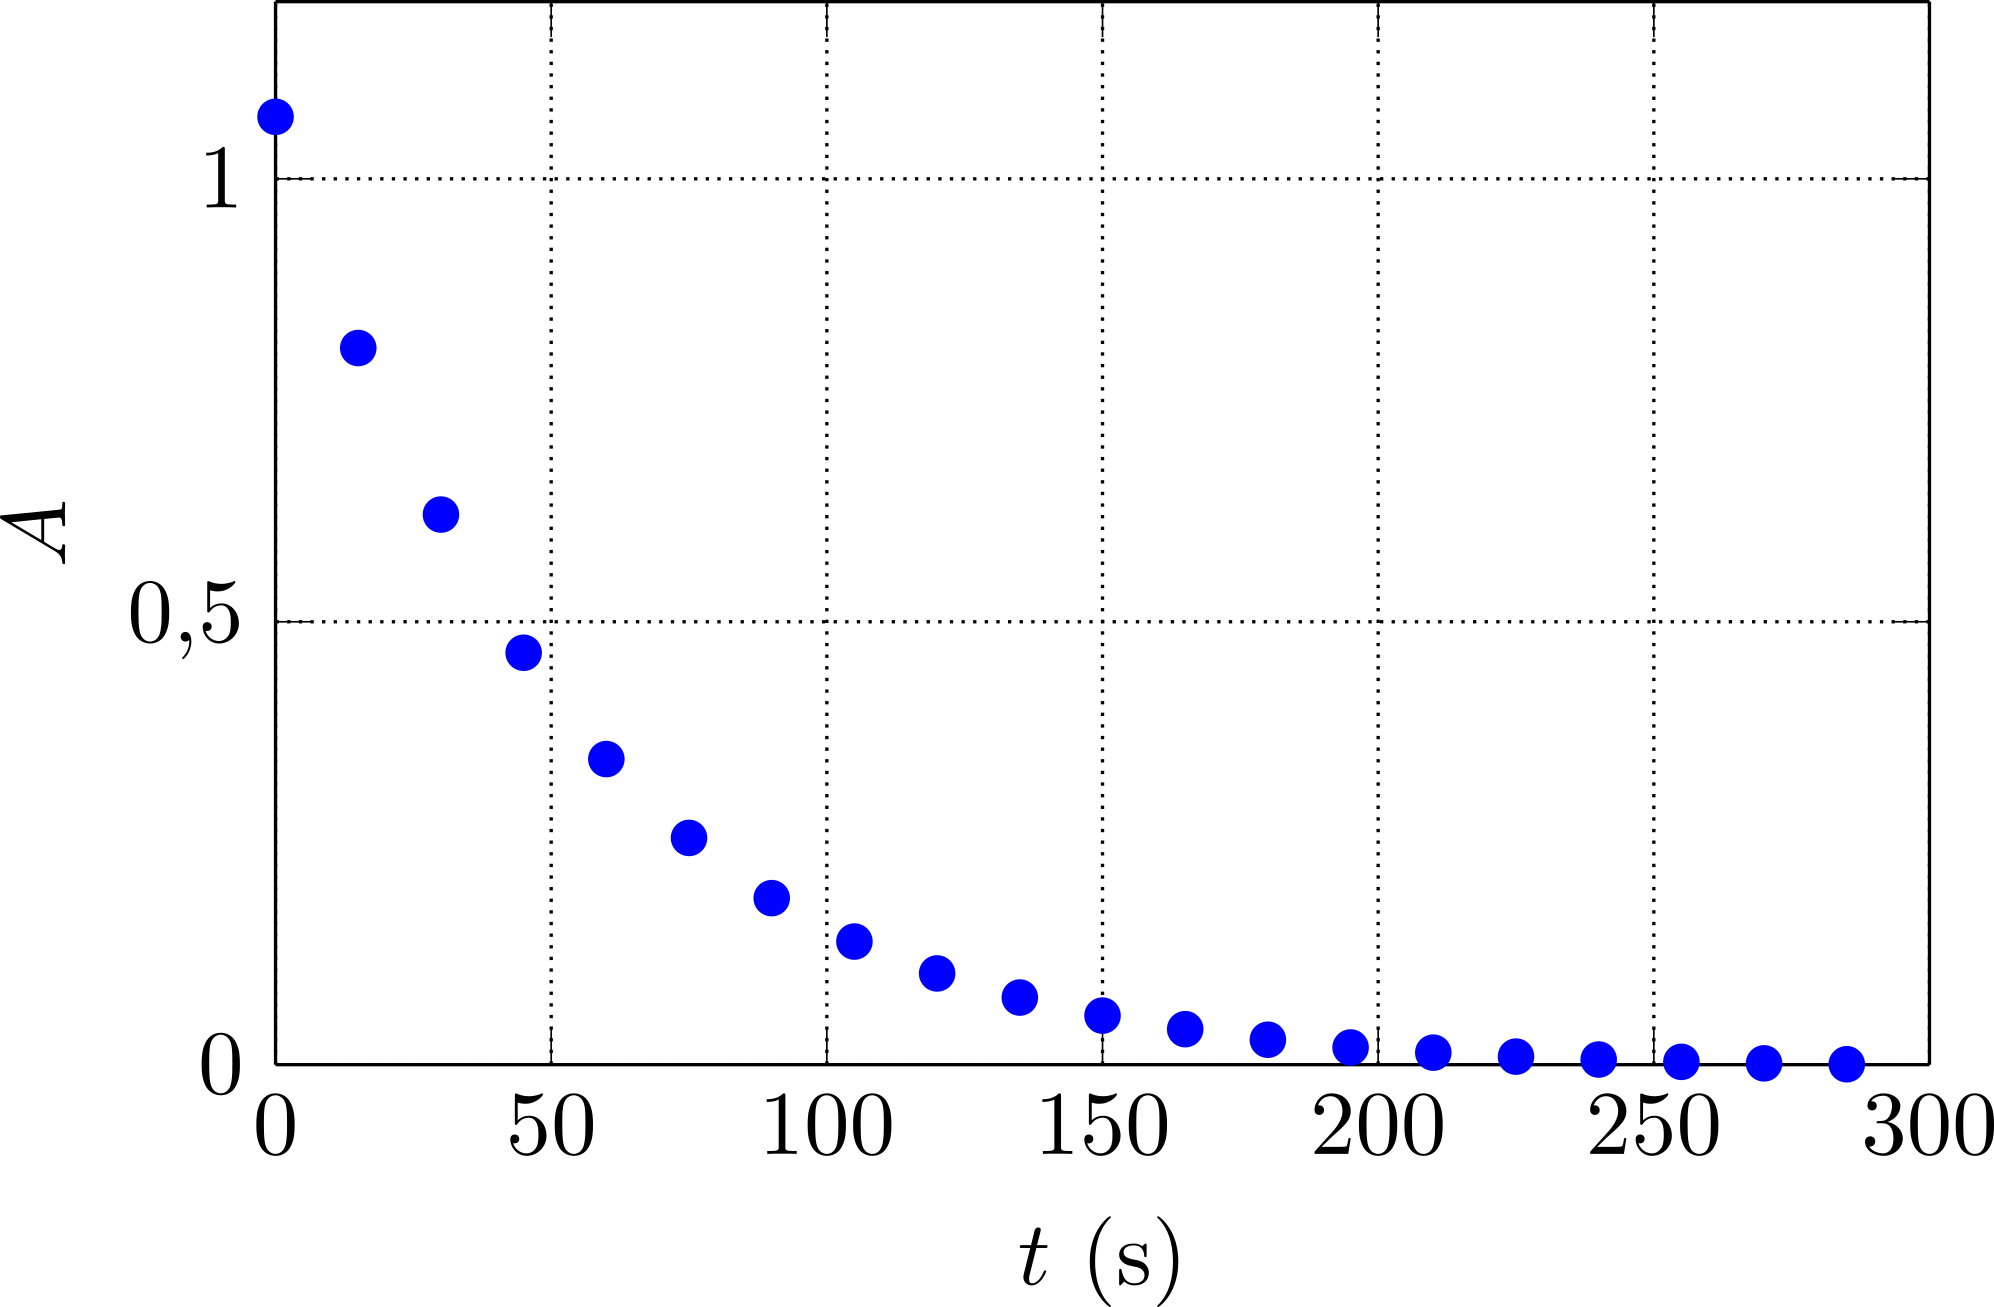
\includegraphics[width=\linewidth]{ph_evol-a}
	\end{center}
\end{minipage}
\begin{minipage}{0.49\linewidth}
	\begin{center}
		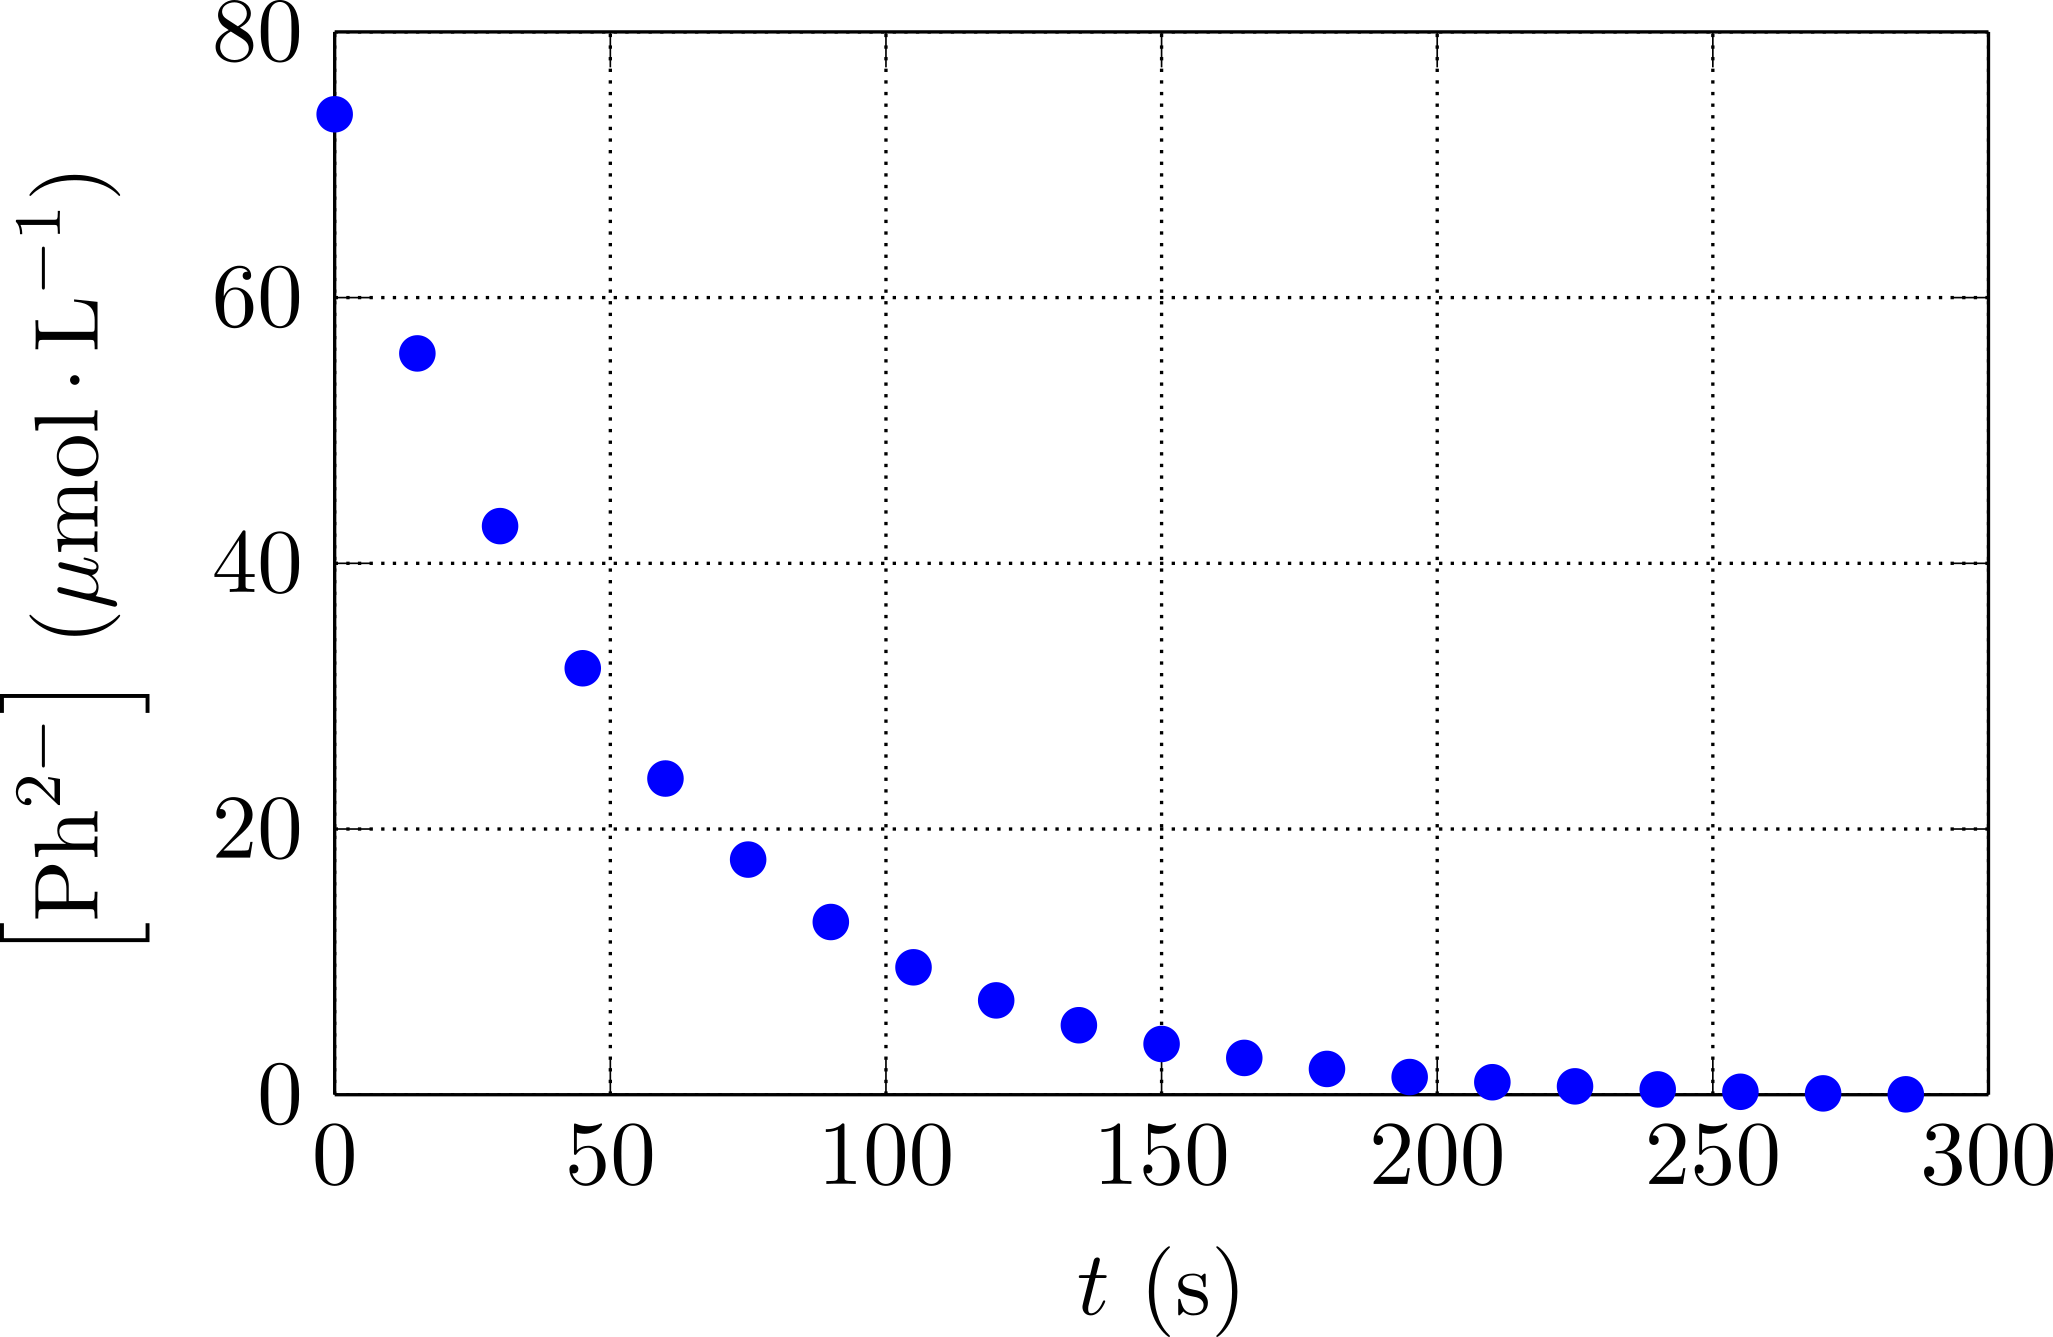
\includegraphics[width=\linewidth]{ph_evol-b}
	\end{center}
\end{minipage}

On établit le tableau d'avancement~:

\begin{center}
	\def\rhgt{0.50}
	\centering
	\begin{tabularx}{\linewidth}{|l|c||YdYdY|}
		\hline
		\multicolumn{2}{|c||}{
			$\xmathstrut{\rhgt}$
		\textbf{Équation}}     &
		$\ce{Ph^{2-}\aqu{}}$   & $+$     &
		$\ce{HO^{-}\aqu{}}$    & $=$     &
		$\ce{PhOH^{3-}\aqu{}}$             \\
		\hline
		$\xmathstrut{\rhgt}$
		Initial                & $x = 0$ &
		$[\ce{Ph^{2-}}]_0$     & \vline  &
		$[\ce{HO^{-}}]_0$      & \vline  &
		$0$                                \\
		\hline
		$\xmathstrut{\rhgt}$
		Interm.                & $x$     &
		$[\ce{Ph^{2-}}]_0 - x$ & \vline  &
		$[\ce{HO^{-}}]_0 - x$  & \vline  &
		$x$                                \\
		\hline
	\end{tabularx}
\end{center}

\leftcentersright{%
D'où on tire
}{%
\psw{
$[\ce{Ph^{2-}}] = [\ce{Ph^{2-}}]_0 - x \Lra x = [\ce{Ph^{2-}}]_0 - [\ce{Ph^{2-}}]$
}
}{%
donnant la courbe~:
}

\begin{center}
	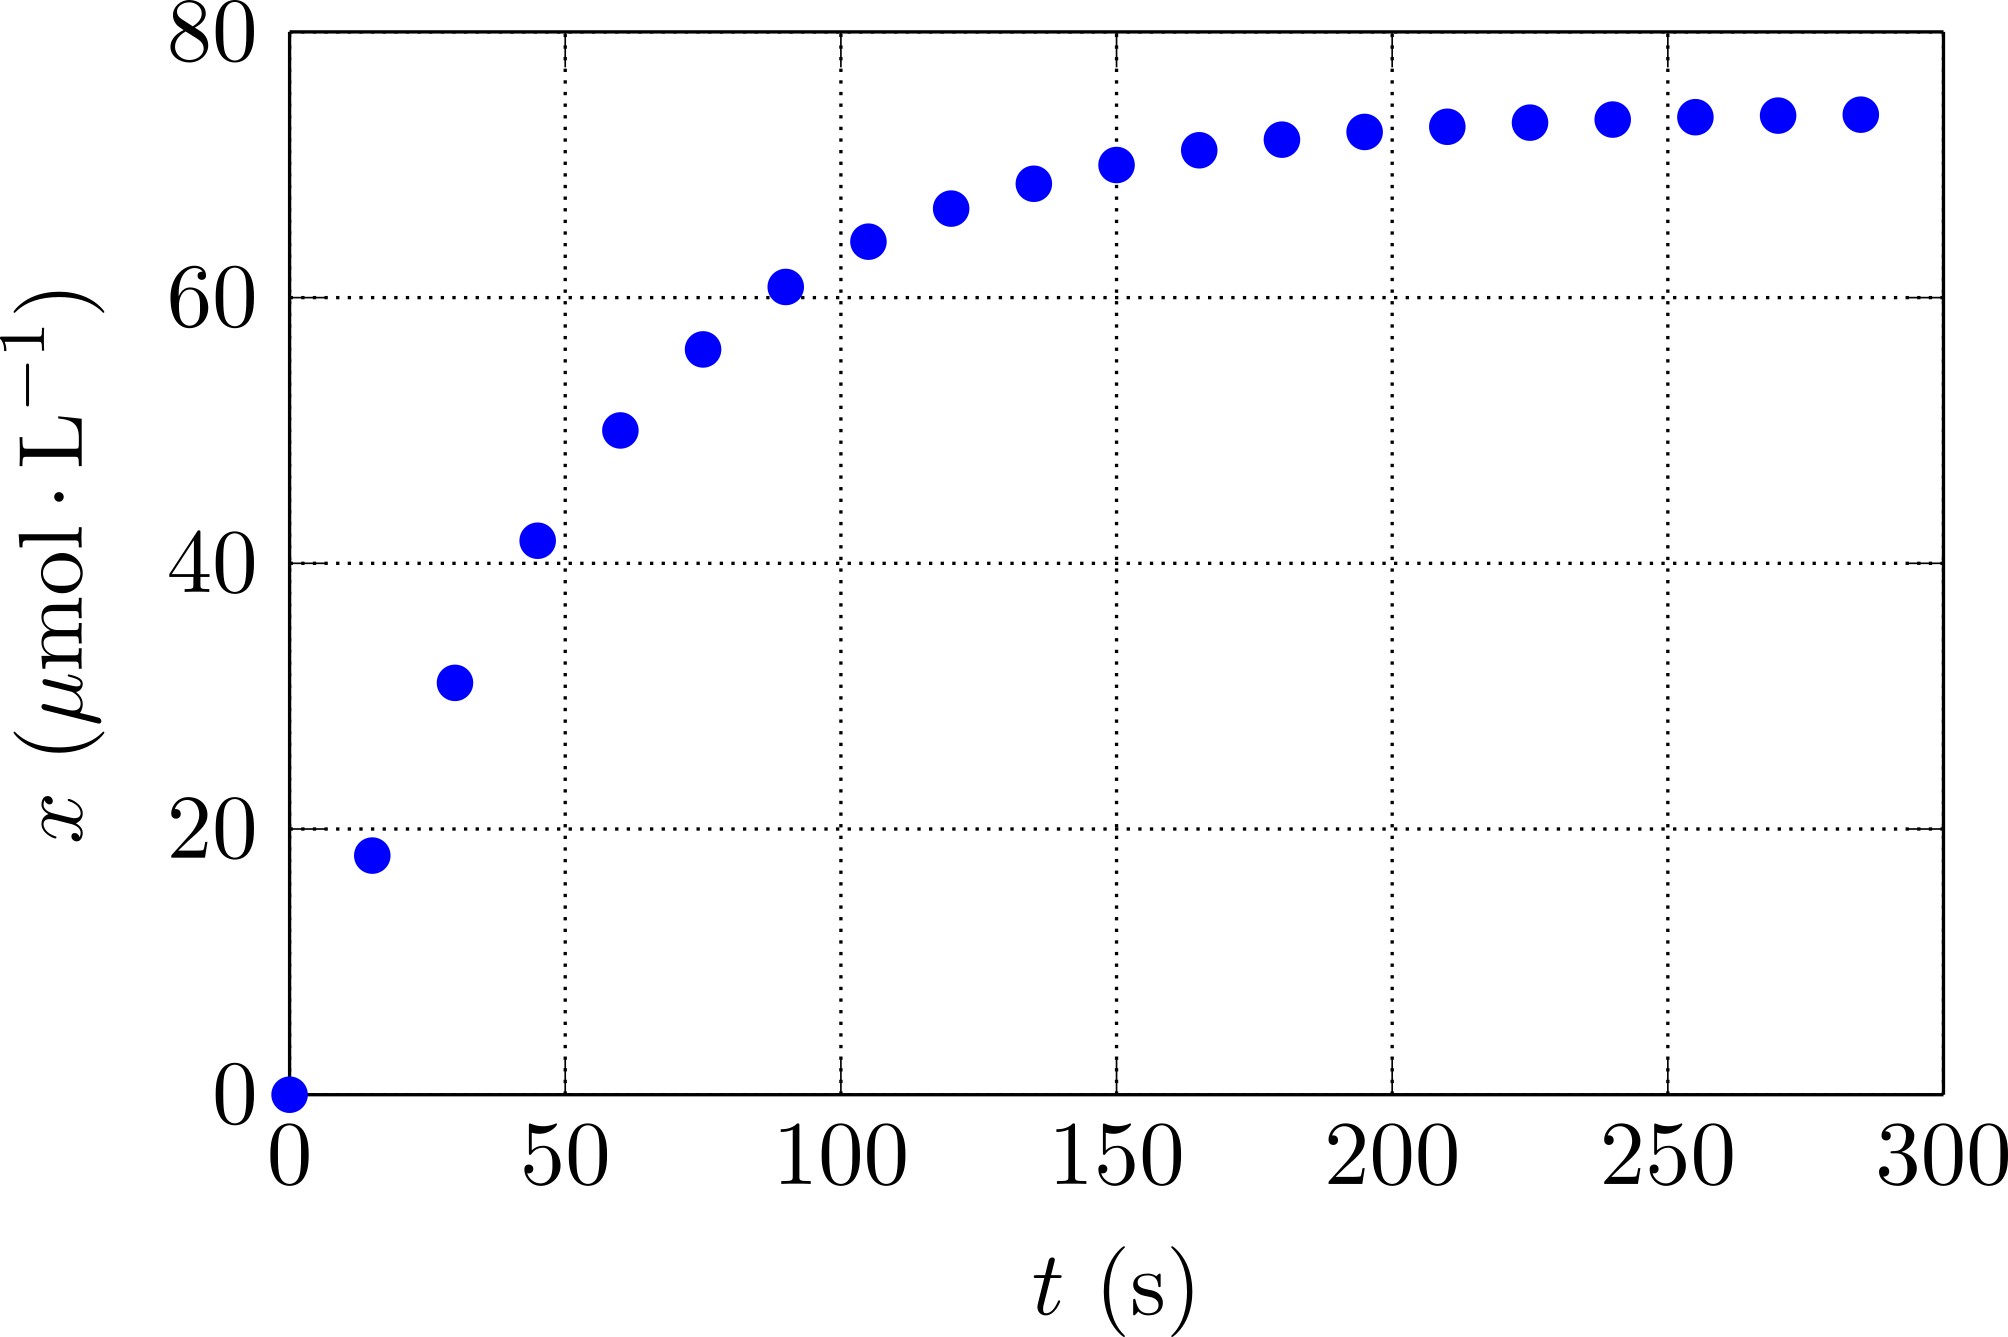
\includegraphics[width=.5\linewidth]{ph_evol-c}
\end{center}

L'avancement augmente bien avec le temps, mais on voit qu'il augmente
\textbf{plus vite au début} de la réaction qu'à la fin. En prenant la
\textbf{dérivée} de cette évolution, on trouve donc la \textbf{vitesse de
	l'avancement} $v = \dd x/\dd t$. Tracer cette grandeur en fonction du temps puis
en fonction de $[\ce{Ph^{2-}}]$ donne~:

\begin{minipage}{0.49\linewidth}
	\begin{center}
		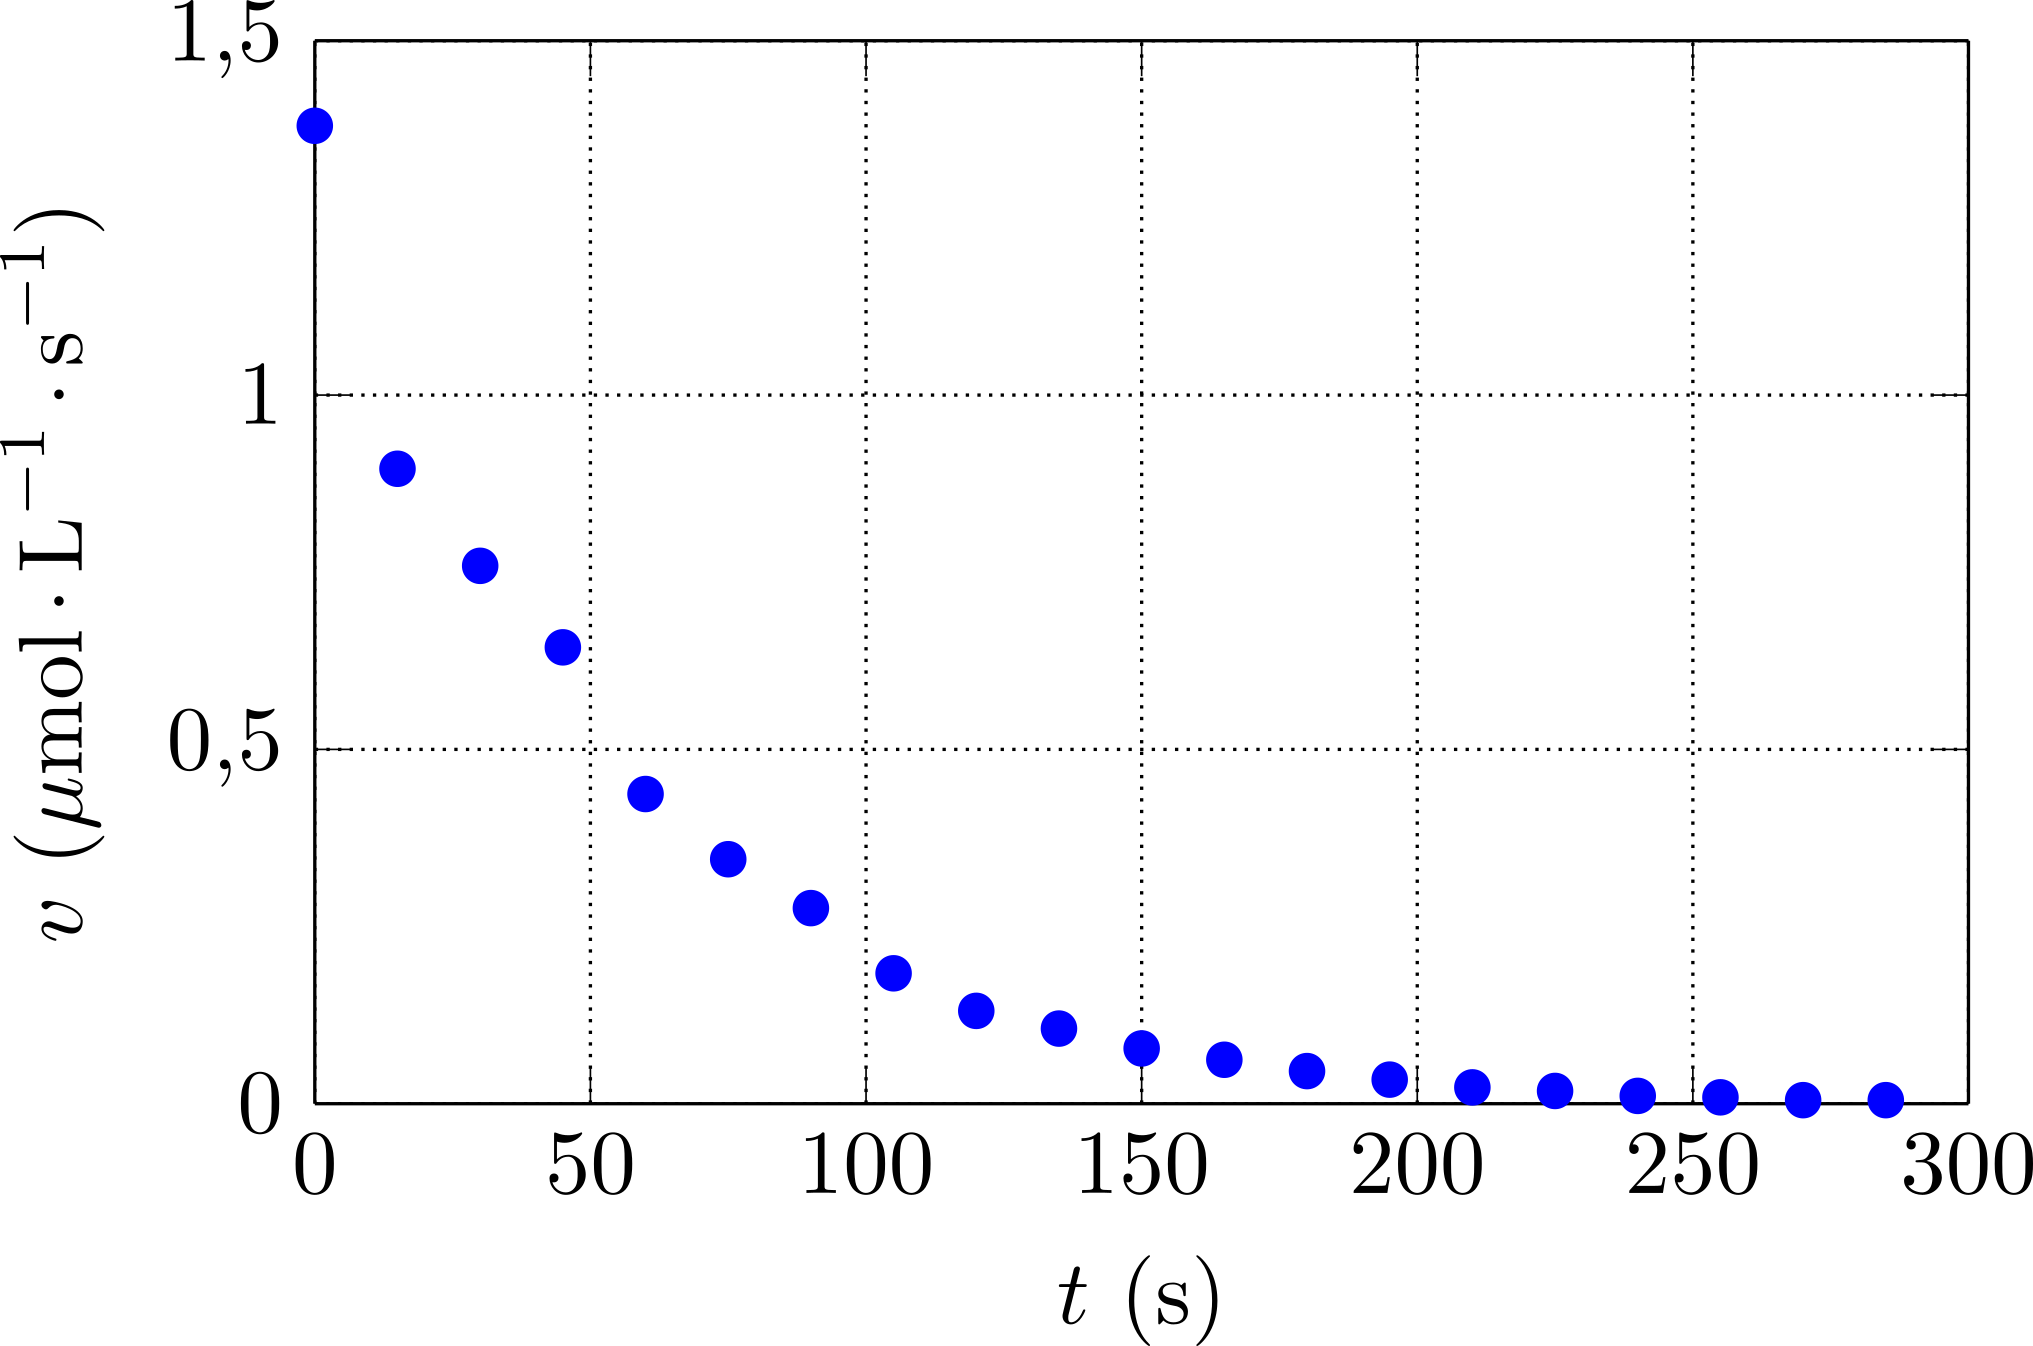
\includegraphics[width=\linewidth]{ph_evol-d}
	\end{center}
\end{minipage}
\begin{minipage}{0.49\linewidth}
	\begin{center}
		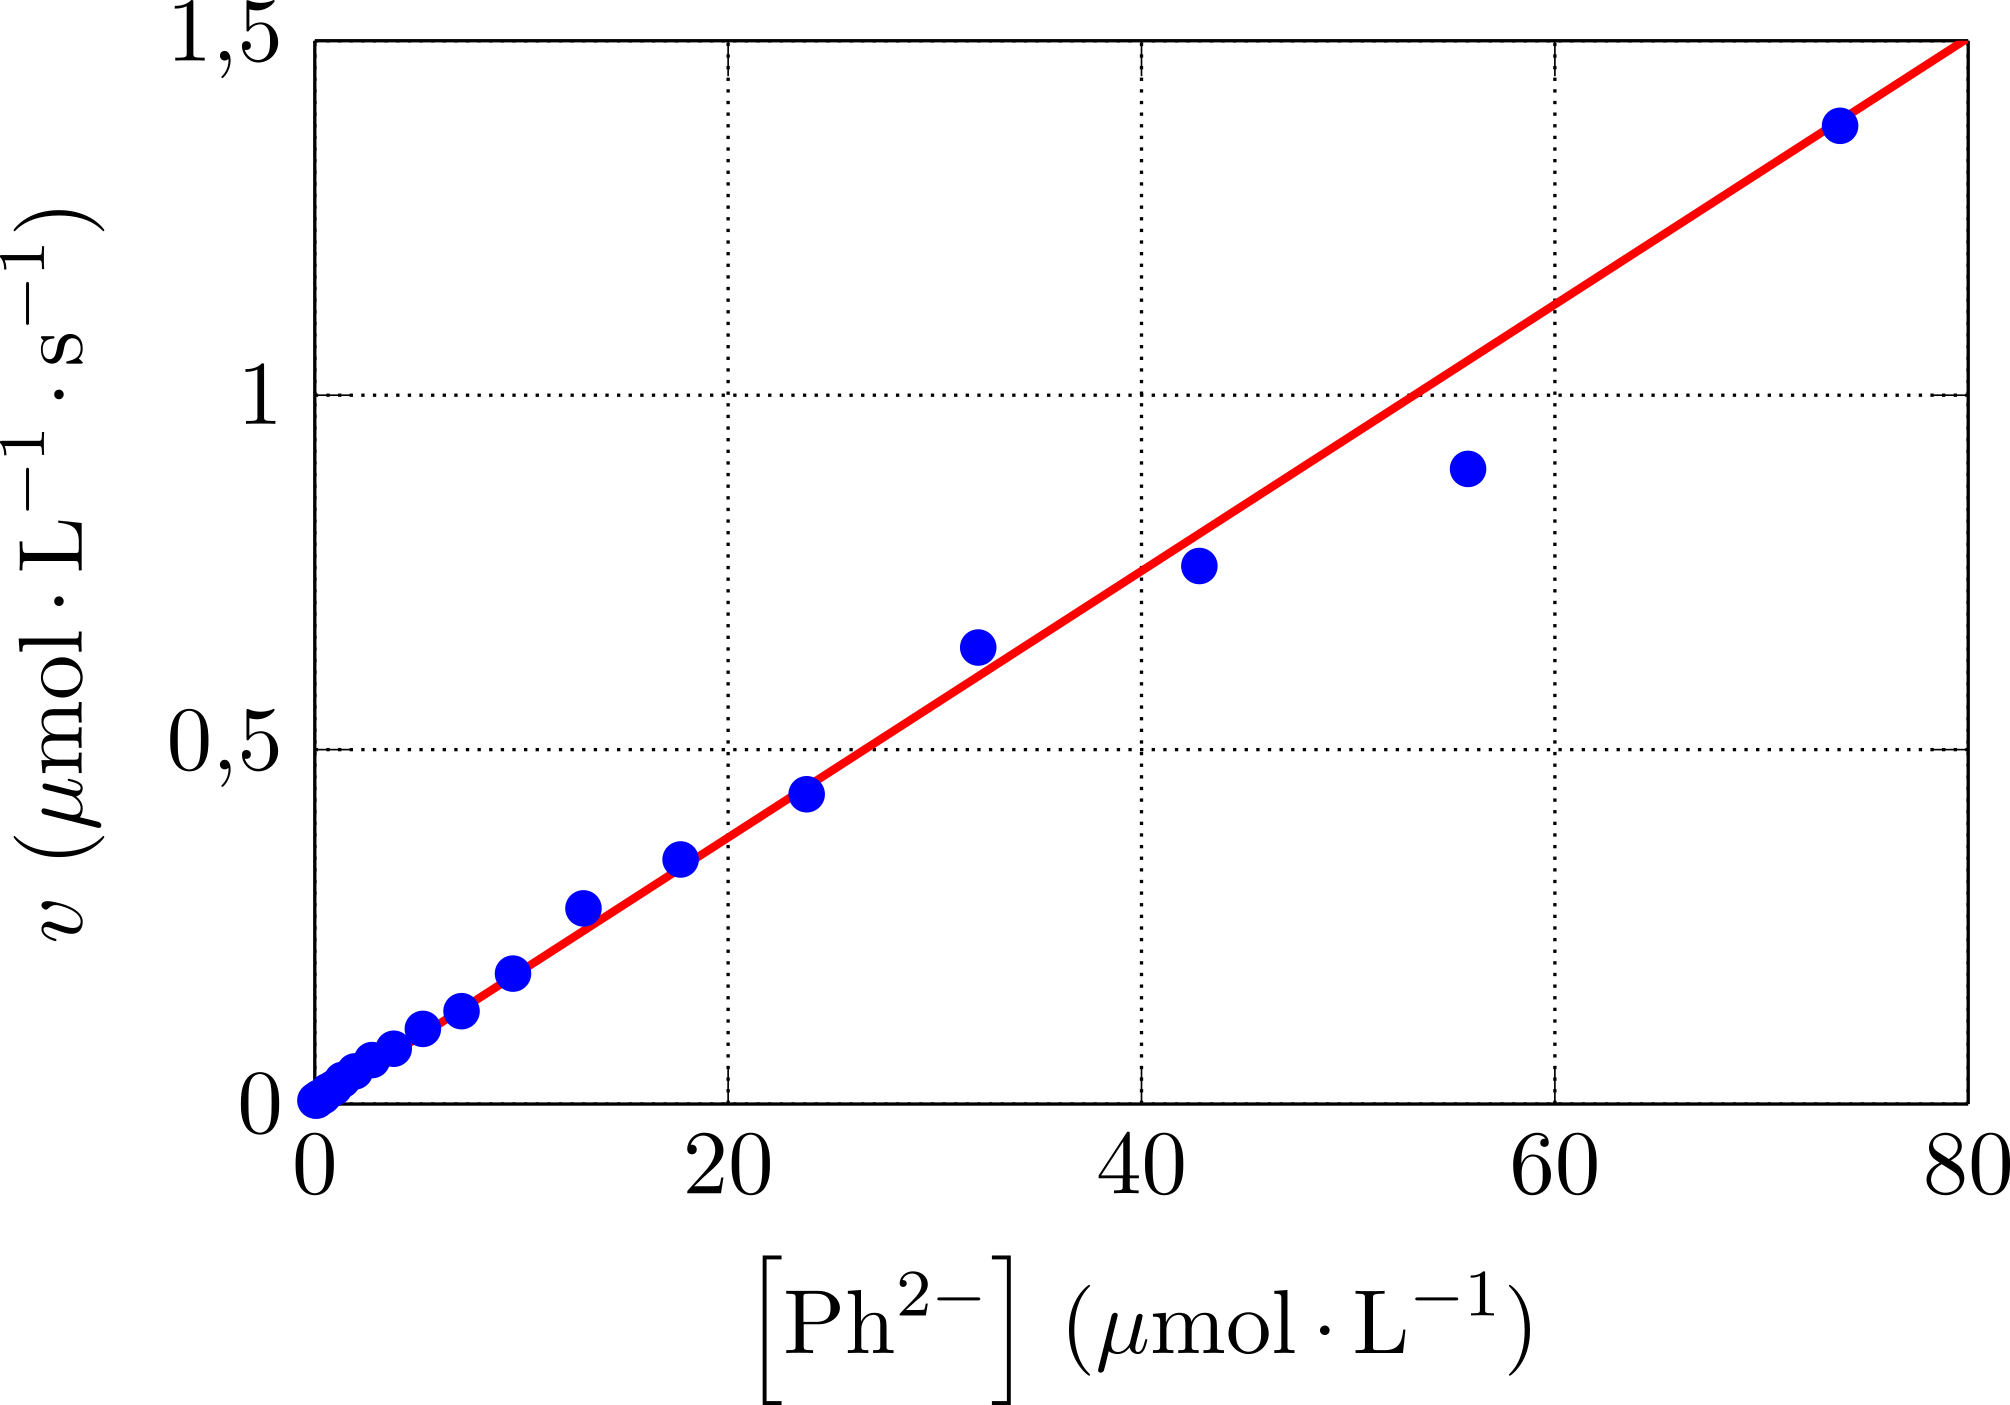
\includegraphics[width=\linewidth]{ph_evol-e}
	\end{center}
\end{minipage}

Ainsi, \textbf{dans cet exemple} de réaction et avec $[\ce{HO^{-}}]_0 =
	\SI{1}{mol.L^{-1}}$, on a $v = k[\ce{Ph^{2-}}]$ avec $k =
	\SI{1.88e-2}{s^{-1}}$. La même étude avec $[\ce{HO^{-}}]_0 =
	\SI{0.4}{mol.L^{-1}}$ donne $k = \SI{7.0e-3}{s^{-1}}$, c'est-à-dire une vitesse
plus faible que précédemment.

\subsection{Facteurs cinétiques}

À partir de l'expérience précédente, on note qu'une \textit{augmentation de la
	concentration de soude accélère la réaction}. L'avancement a atteint la moitié de
sa valeur finale en \SI{38}{s} avec une concentration de $\SI{1.0}{mol.L^{-1}}$,
et en \SI{1}{min} \SI{30}{s} pour une concentration de $\SI{0.4}{mol.L^{-1}}$~:
c'est donc un \textbf{facteur cinétique}. On en recense 4~:

\begin{tcb}[label=def:factciné, breakable](defi){Facteurs cinétiques}
	Plusieurs facteurs influencent la vitesse d'une réaction donnée~:
	\begin{itemize}
		\item
		      \psw{
			      La concentration initale des réactifs~: $[\ce{R_i}]_0 \nearrow
				      \Rightarrow v \nearrow$~;
		      }
		\item
		      \psw{
			      La température~: $t \nearrow \Rightarrow v \nearrow$~;
		      }
		\item
		      \psw{
			      La présence de catalyseurs, qui permettent d'accélérer une
			      réaction sans l'altérer~;
		      }
		\item
		      \psw{
			      Le solvant utilisé.
		      }
	\end{itemize}
\end{tcb}

On peut comprendre cela avec la notion de \textbf{choc efficace}~: pour qu'une
réaction ait lieu, il faut que deux molécules entrent en contact et ce avec
suffisamment d'énergie. La vitesse de réaction dépend donc de la probabilité que
deux molécules se choquent, et que ce choc soit efficace.
\begin{itemize}
	\item
	      \psw{
		      Plus concentration $\nearrow$, plus la probabilité qu'un réactif
		      entre en contact avec un autre $\nearrow$.
	      }
	\item
	      \psw{
		      Plus la température $\nearrow$, plus la vitesse des molécules $\nearrow$~:
		      la fréquence des chocs augmente et la probabilité que ces chocs
		      soient efficaces aussi.
	      }
\end{itemize}

\begin{tcb}(impo)<lfnt>{}
	\textbf{Attention}~: beaucoup de réactions ne sont pas de simples collisions
	entre deux réactifs, mais sont une longue suite de processus et l'équation-bilan
	n'en est qu'une synthèse.
\end{tcb}

\section{Vitesse(s) de réaction}
\subsection{Hypothèses de travail}
Pour la définition formelle de l'étude de la cinétique, on pose le cadre
d'étude. Les systèmes physico-chimiques considérés seront tous~:
\begin{itemize}
	\item \psw{
		      \textbf{fermés} (pas d'échange de matière)~;
	      }
	\item \psw{
		      \textbf{isothermes} (température constante)~;
	      }
	\item \psw{
		      \textbf{isobares} (pression constante)~;
	      }
	\item \psw{
		      \textbf{homogènes} (avec une unique phase).
	      }
	\item \psw{
		      et surtout \textbf{à volume constant}.
	      }
\end{itemize}

\subsection{Vitesse de réaction}

Pour définir la vitesse d'une réaction de manière satisfaisante, elle doit être
\textbf{indépendante de l'espèce chimique suivie}~: pour caractériser la
réaction on utilisera donc l'\textbf{avancement} de la réaction. Il aussi
souhaitable que la vitesse soit intensive, donc ne dépende pas de la taille du
système~: on s'intéresse donc à l'avancement \textbf{volumique} $x = \xi/V$.
Ainsi,
\begin{tcb}[label=def:vreac, sidebyside, righthand ratio=.3](defi)
	{Vitesse de réaction}
	On définit la vitesse d'une réaction par
	\psw{
		\[\boxed{
				v\ftn{
					On trouve aussi parfois la notation $r$ pour la vitesse, pour la
					différencier de la vitesse en mécanique et ne pas confondre $x$ avec
					la position d'un corps massique.
				}
				= \dv{x}{t}} \qavec \boxed{x = \frac{\xi}{V}}\]
	}
	\tcblower
	\tcbsubtitle{\fatbox{Unité}}
	\psw{
	$\si{mol.L^{-1}.s^{-1}}$
	}
\end{tcb}

\subsection{Vitesses de formation/disparition}

En plus de la vitesse de réaction, on peut en effet définir la vitesse de
formation d'un produit, ou de disparition d'une espèce.
\newpage
\begin{tcb}[label=def:vfordisp, heart](defi){Vitesses de formation et disparition}
	\leftcenters{%
		Pour une réaction
	}{%
		$
			\ce{\alpha_1R_1 + \alpha_2R_2} +…
			=
			\ce{\beta_1P_1 +\beta_2P_2}+…
		$
	}
	\begin{isd}
		La vitesse de formation d'un produit est
		\psw{
			\[\boxed{v_{f,\ce{P}} = \dv{[\ce{P}]}{t}}\]
		}
		\tcblower
		La vitesse de disparition d'un réactif est
		\psw{
			\[\boxed{v_{f,\ce{R}} = -\dv{[\ce{R}]}{t}}\]
		}
		\textbf{Attention au signe «~-~»~}: le réactif disparaît, mais la \textbf{vitesse} doit
		être \textbf{positive}.
	\end{isd}
\end{tcb}

En reprenant l'exemple précédent, on a bien
\begin{flalign*}
	v_{d,\ce{HO^{-}}}    & =
	\psw{
		- \dv{[\ce{HO^{-}}]}{t} =
		- \dv{([\ce{HO^{-}}]_0 - x)}{t} =
		-0 + \dv{x}{t} =
		v
	}                    &
	\\
	v_{f,\ce{PhOH^{3-}}} & =
	\psw{
		\dv{[\ce{PhOH^{3-}}]}{t} =
		\dv{x}{t} =
		v
	}                    &
\end{flalign*}

D'un manière plus générale, à partir de l'écriture algébrique de la réaction, on
a
\psw{
	\[0 = \sum_{i=1}^{N} \nu_i {\ce{X}}_i \qavec \xi = \frac{n_i - n_i^0}{\nu_i}\]
}
En divisant par $V$ pour avoir l'avancement volumique et en prenant la dérivée,
on a donc
\begin{tcb}[label=prop:vreacfordisp](prop){Lien entre vitesse de réaction et de
			formation/disparition}
	\psw{
	\[
		\boxed{v = \frac{1}{\nu_i} \dv{[{\ce{X}}_i]}{t}}
		\Lra
		\boxed{v = -\frac{1}{\nu_i}v_{f,\ce{R}}
		=
		\frac{1}{\nu_i}v_{f,\ce{P}}}
	\]
	}
\end{tcb}

En effet, avec un tableau d'avancement général on aurait
\begin{center}
	\def\rhgt{0.35}
	\centering
	\begin{tabularx}{\linewidth}{|l|c||YdYdYdY|}
		\hline
		\multicolumn{2}{|c||}{
			$\xmathstrut{\rhgt}$
		\textbf{Équation}}          &
		$a\ce{A}$                   & $+$     &
		$b\ce{B}$                   & $\ra$   &
		$c\ce{C}$                   & $+$     &
		$d\ce{D}$                               \\
		\hline
		$\xmathstrut{\rhgt}$
		Initial                     & $x = 0$ &
		$c_{\ce{A}}^{0}$            & \vline  &
		$c_{\ce{B}}^{0}$            & \vline  &
		$c_{\ce{C}}^{0}$            & \vline  &
		$c_{\ce{D}}^{0}$                        \\
		\hline
		$\xmathstrut{\rhgt}$
		Interm.                     & $x$     &
		\psw{$c_{\ce{A}}^{0} - ax$} & \vline  &
		\psw{$c_{\ce{B}}^{0} - bx$} & \vline  &
		\psw{$c_{\ce{C}}^{0} + cx$} & \vline  &
		\psw{$c_{\ce{D}}^{0} + dx$}             \\
		\hline
	\end{tabularx}
\end{center}
\begin{flalign*}
	\Ra
	v_{d, \ce{A}} & =
	\psw{
		- \dv{[\ce{A}]}{t} = - \dv{(c_{\ce{A}} - ax)}{t} = av
	}             &
	\\
	\qet
	v_{f, \ce{C}} & =
	\psw{
		\dv{[\ce{C}]}{t} = \dv{(c_{\ce{C}} + cx)}{t} = cv
	}             &
	\vspace{-15pt}
\end{flalign*}

\begin{tcb}[width=\linewidth, breakable](appl){Exercice}
	Écrire $v$ en fonction des concentrations pour la réaction
	\[
		\ce{6H^{+}\aqu{} + 5Br^{-}\aqu{} + BrO3^{-}\aqu{}
			=
			3Br2\aqu{} + 2H2O\liq{}}
	\]
	\tcblower
	\psw{
		D'après la propriété précédente, on a
		\[
			v = - \frac{1}{6} \dv{[\ce{H+}]}{t}
			= - \frac{1}{5} \dv{[\ce{Br-}]}{t}
			= - \dv{[\ce{BrO3-}]}{t}
			= \frac{1}{3} \dv{[\ce{Br2}]}{t}
		\]
	}
	\vspace{-15pt}
\end{tcb}

\section{Concentration et ordre de réaction}
\subsection{Ordre de la réaction}
\textit{A priori}, il n'y a \textit{pas de relation simple} permettant de
déterminer la vitesse d'une réaction en fonction des paramètres
physico-chimiques du systèmes. Cependant, il y a certaines réactions qui ont une
expression simple, comme on l'a vu en introduction. Prenons une réaction de la
forme
\psw{
\[
	a\ce{A} + b\ce{B} = c\ce{C} + d\ce{D}
	\Longleftrightarrow
	\sum_{i=1}^{p} \left| \nu_i \right| {\ce{R}}_i = \sum_{i=p+1}^{N} \nu_i {\ce{P}}_i
\]
}
\vspace{-15pt}
\begin{tcb}*[label=def:ordre](defi)"ror"{Ordre de réaction}
	Une telle réaction est dite \textbf{admettant un ordre} si sa vitesse peut
	s'écrire sous la forme
	\psw{
	\[
		\boxed{v = k[\ce{A}]^p[\ce{B}]^q}
		\Longleftrightarrow
		\boxed{v = k \prod_{i=1}^{p}[{\ce{R}}_i]^{m_i}}
	\]
	}
	On définit alors~:
	\begin{itemize}
		\item \psw{
			      $k$ la constante de vitesse, dont \textbf{l'unité dépend de
				      $p$ et $q$}~;
		      }
		\item \psw{
			      $p$ et $q$ (ou $m_i$) sont les \textbf{ordres partiels} de
			      la réaction~;
		      }
		\item \psw{
			      $p + q$ (ou $m = \sum m_i$) est \textbf{l'ordre global}
			      de la réaction.
		      }
	\end{itemize}
	On s'arrangera pour que $p$ et $q$ soient en général des entiers ou
	demi-entiers.
\end{tcb}

\begin{tcb}*[cnt, bld](prop)"bomb"{Attention}
	\begin{itemize}
		\item La vitesse d'une réaction possédant un ordre ne s'exprime qu'en fonction des
		      réactifs~!!
		\item $p$ et $q$ n'ont \textit{a priori} rien à
		      voir avec $\nu_i$.
	\end{itemize}
\end{tcb}

\subsection{Ordre initial et ordre courant}

Certaines réactions ont un ordre à tout instant de la réaction, appelé
\textbf{ordre courant}, d'autre peuvent n'avoir qu'un \textbf{ordre initial},
c'est-à-dire valable uniquement aux premiers instants. Par exemple, la réaction
\psw{
	\[\ce{Br2\gaz{} + H2\gaz{} = 2HBr\gaz{}}\]
}
a empiriquement une loi de vitesse de la forme
\psw{
	\[
		v = \frac{k[\ce{H2}]\times[\ce{Br2}]^{1/2}}
		{1+k' \frac{[\ce{HBr}]}{[\ce{Br2}]}}
	\]
}
\noindent
C'est une réaction qui est \textbf{sans ordre}, puisqu'elle ne s'exprime pas
comme un produit des concentrations des réactifs à certaines puissances et fait
intervenir la concentration en produit.
\smallbreak
Cependant, si on part avec $[\ce{HBr}]_0 =
	0$, aux premiers instants de la réaction on a $[\ce{HBr}] \ll [\ce{Br2}]$, et on
peut négliger le dénominateur. Ainsi, la loi de vitesse devient~:
\psw{
	\[v \Sim_{t\to 0} k [\ce{H2}][\ce{Br2}]^{1/2}\]
}
On dit donc que cette réaction est sans ordre mais admet un \textbf{ordre initial}.

\subsection{Cas particulier des réactions simples}
\subsubsection{Définition}
\begin{tcb}[label=def:reacsimple](defi){Réaction simple}
	\begin{itemize}
		\bitem{Réaction simple}~:
		\psw{
			lorsque la transformation chimique des
			réactifs aux produits s'effectue en une unique étape élémentaire, un
			\textbf{unique acte chimique}.
		}
		\bitem{Acte chimique}~:
		\psw{
			étape élémentaire. Réaction chimique
			qui décrit les collisions qui se passent réellement au \textbf{niveau
				moléculaire}.
		}
		\bitem{Réaction composée}~:
		\psw{
			par opposition, passage par des \textbf{intermédiaires} réactionnels (IR).
		}
		\bitem{intermédiaire réactionnel}~:
		\psw{
			espèce participant à un
			mécanisme réactionnel et qui n'est \textbf{ni un réactif, ni un produit}
			dans l'équation-bilan de la réaction.
		}
	\end{itemize}
	\leftcenters{%
		Exemple~:
	}{%
		\psw{
			réactif1 $\ra$ IR1 + réactif2 $\ra$ IR2 $\ra$ IR3 $\ra$ produit
		}
	}
\end{tcb}

\subsubsection{Loi de \textsc{Van't Hoff}}
\begin{tcb}*[label=loi:vanthoff](loi)"ror"{Loi de \textsc{Van't Hoff}}
	Pour une \textbf{réaction simple}, les \textbf{ordres partiels} sont égaux
	au \textbf{coefficients stœchiométriques \underline{arithmétiques}}
	(c'est-à-dire positifs)~:
	\psw{
	\[
		\boxed{v = k[{\ce{A}}]^{\left| \nu_{\ce{A}} \right|}
				[{\ce{B}}]^{\left| \nu_{\ce{B}} \right|}}
		\Longleftrightarrow
		\boxed{v = k\prod_{i=1}^{p}[{\ce{R}}_i]^{\left| \nu_i \right|}}
	\]
	}
\end{tcb}

\subsection{Autres cas particuliers}
\subsubsection{Dégénérescence de l'ordre}
D'une manière générale, quand il y a plusieurs réactifs l'expression de la
vitesse dépend d'un grand nombre de variables, même si elles sont toutes reliées
par $\xi$. Il est alors \textbf{impossible de déterminer indépendamment chacun
	des ordres partiels, et seul l'ordre global est accessible}. Pour les
déterminer, on utilise une méthode essentielle à la cinétique chimique~: la
dégénérescence de l'ordre.
\bigbreak
L'idée de la dégénérescence de l'ordre, c'est de réussir à n'avoir qu'un seul
réactif dont la concentration évolue avec le temps~; pour cela, il suffit
d'introduire les autres réactifs en large excès, auquel cas leurs concentrations
seront proche de leur concentration initiale. Dans le cas de deux réactifs A et
B, si on introduit A en excès on aura
\psw{
	\[[\ce{A}](t) \approx [\ce{A}]_0\]
}
et la loi de vitesse est alors
\[
	\boxed{
	\psw{
	v =
	k[\ce{A}]^{p}[\ce{B}]^{q} =
	\underbracket[1pt]{k[\ce{A}]_0{}^{p}}_{= \cte}[\ce{B}]^{q} =
	k_{\rm app}[\ce{B}]^{q}
	}
	}
\]

On introduit alors $k_{\rm app}$ la \textbf{constante de vitesse apparente}, et
l'ordre global apparent est donc égal à l'ordre partiel $q$. C'est le
principe utilisé en introduction, où la réaction
\[\ce{Ph^{2-}\aqu{} + HO^{-}\aqu{} = PhOH^{-3}\aqu{}}\]
a une vitesse de réaction qui peut s'écrire
\[v = k[\ce{HO^{-}}]^{p}[\ce{Ph^{2-}}]^{q}\]

mais où nous avions introduit $\SI{1.0}{mol.L^{-1}}$ d'hydroxyde contre
$\SI{70}{\micro mol.L^{-1}}$ de phénolphtaléine~: on avait donc $k_{\rm app} =
	k[\ce{HO^{-}}]_0^{p}$. Vous pouvez vérifier que le rapport des
concentrations initiales en hydroxyde indiquées est égal au rapport des
constantes de vitesse données.

\begin{tcb}[label=prop:dege, bld, cnt](ror){Dégénérescence de l'ordre}
	Pour une réaction admettant un ordre, en ajoutant tous les réactifs en excès
	sauf 1, on a accès à l'ordre partiel de ce réactif.
\end{tcb}

\subsubsection{Proportions stœchiométriques}
\leftcenters{%
Soit la réaction
}{%
$
	a{\ce{A}} + b{\ce{B}}
	=
	c{\ce{C}} +d{\ce{D}}
$
}
\smallbreak
\noindent
si A et B sont introduits en proportions stœchiométriques, alors on peut
noter initialement
\psw{
	\[
		[{\ce{A}}]_0 = ac_0
		\qet
		[{\ce{B}}]_0 = bc_0
	\]
}
et à tout instant
\psw{
	\[
		\boxed{
			[{\ce{A}}] = a (c_0 - x)
			\qet
			[{\ce{B}}] = b (c_0 - x)
		}
	\]
}
On peut donc factoriser la loi de vitesse~:
\psw{
	\begin{gather*}
		v =
		k \left( a (c_0 - x)\right)^{p}\left( b (c_0 - x)\right)^{q}
		\\\Lra
		\boxed{
		v =
		ka^{p}b^{q} \left(c_0 - x\right)^{p + q}
		}
		\\\Lra
		\boxed{v = k_{\rm app} (c_0 -x)^{m}}
	\end{gather*}
}
avec $m = p + q$ l'ordre global, et $k\ind{app} = ka^{p}b^{q}$ la constante
apparente.

\begin{tcb}[label=prop:stoe, bld, cnt](ror){Proportions stœchiométriques}
	Pour une réaction admettant un ordre, en insérant tous les réactifs dans les
	proportions stœchiométriques, on a accès à l'ordre global de la réaction.
\end{tcb}

\begin{tcb}*(expe)<itc>"trans"{Transition}
	Avec tous ces outils, voyons comment faire en pratique pour des ordres
	courants simples de réaction.
\end{tcb}

\section{Méthodes de résolution}

Dans toutes les situations, un indicateur toujours utilisé en chimie est le
\textbf{temps de demi-réaction}, noté $t_{1/2}$~; on l'a déjà introduit au début
du cours, voici la définition

\begin{tcb}[label=def:tundemi](defi){Temps de demi-réaction}
	On appelle \textbf{temps de demi-réaction} et on note $t_{1/2}$ le temps au
	bout duquel l'avancement a atteint la moitié de sa valeur finale~:
	\psw{
		\[\boxed{\xi(t_{1/2}) = \frac{\xi_f}{2}}\]
	}
\end{tcb}

\subsection{Ordre 0 par rapport à un réactif}

\subsubsection{Hypothèse}
\leftcenters{%
Soit la réaction
}{%
$
	a{\ce{A}} + b{\ce{B}}
	=
	c{\ce{C}} +d{\ce{D}}
$
}
\smallbreak
\leftcenters{%
	Avec la loi de vitesse
}{%
	\psw{
		$v = k [{\ce{A}}]^0 = k$
	}
}

\subsubsection{Unité de $k$}

\psw{
L'unité de $k$ \textbf{dans cette situation} est celle de $v$~: c'est donc des
$\si{mol.L^{-1}.s^{-1}}$.
}

\subsubsection{Équation différentielle}
On souhaite déterminer $[{\ce{A}}](t)$. Avec le lien entre vitesse de réaction et
vitesse de disparition, on a
\psw{
	\[
		\dv{[{\ce{A}}]}{t} = -av
		\Lra
		\boxed{\dv{[{\ce{A}}]}{t} = -ka}
	\]
}

\subsubsection{Résolution}
\leftcenters{%
	On intègre directement~:
}{%
	\psw{
		$[{\ce{A}}](t) = -kat + K$
	}
}
\smallbreak
\noindent
avec $K$ une constante à déterminer par condition initiale. Ici, on a simplement
\psw{
	\begin{gather*}
		[{\ce{A}}](0) = [{\ce{A}}]_0 = K
		\\\Ra
		\boxed{
		[{\ce{A}}](t) = [{\ce{A}}]_0 - kat
		}
	\end{gather*}
	et la concentration diminue \textbf{linéairement avec le temps}.
}

\begin{center}
	\sswitch{
		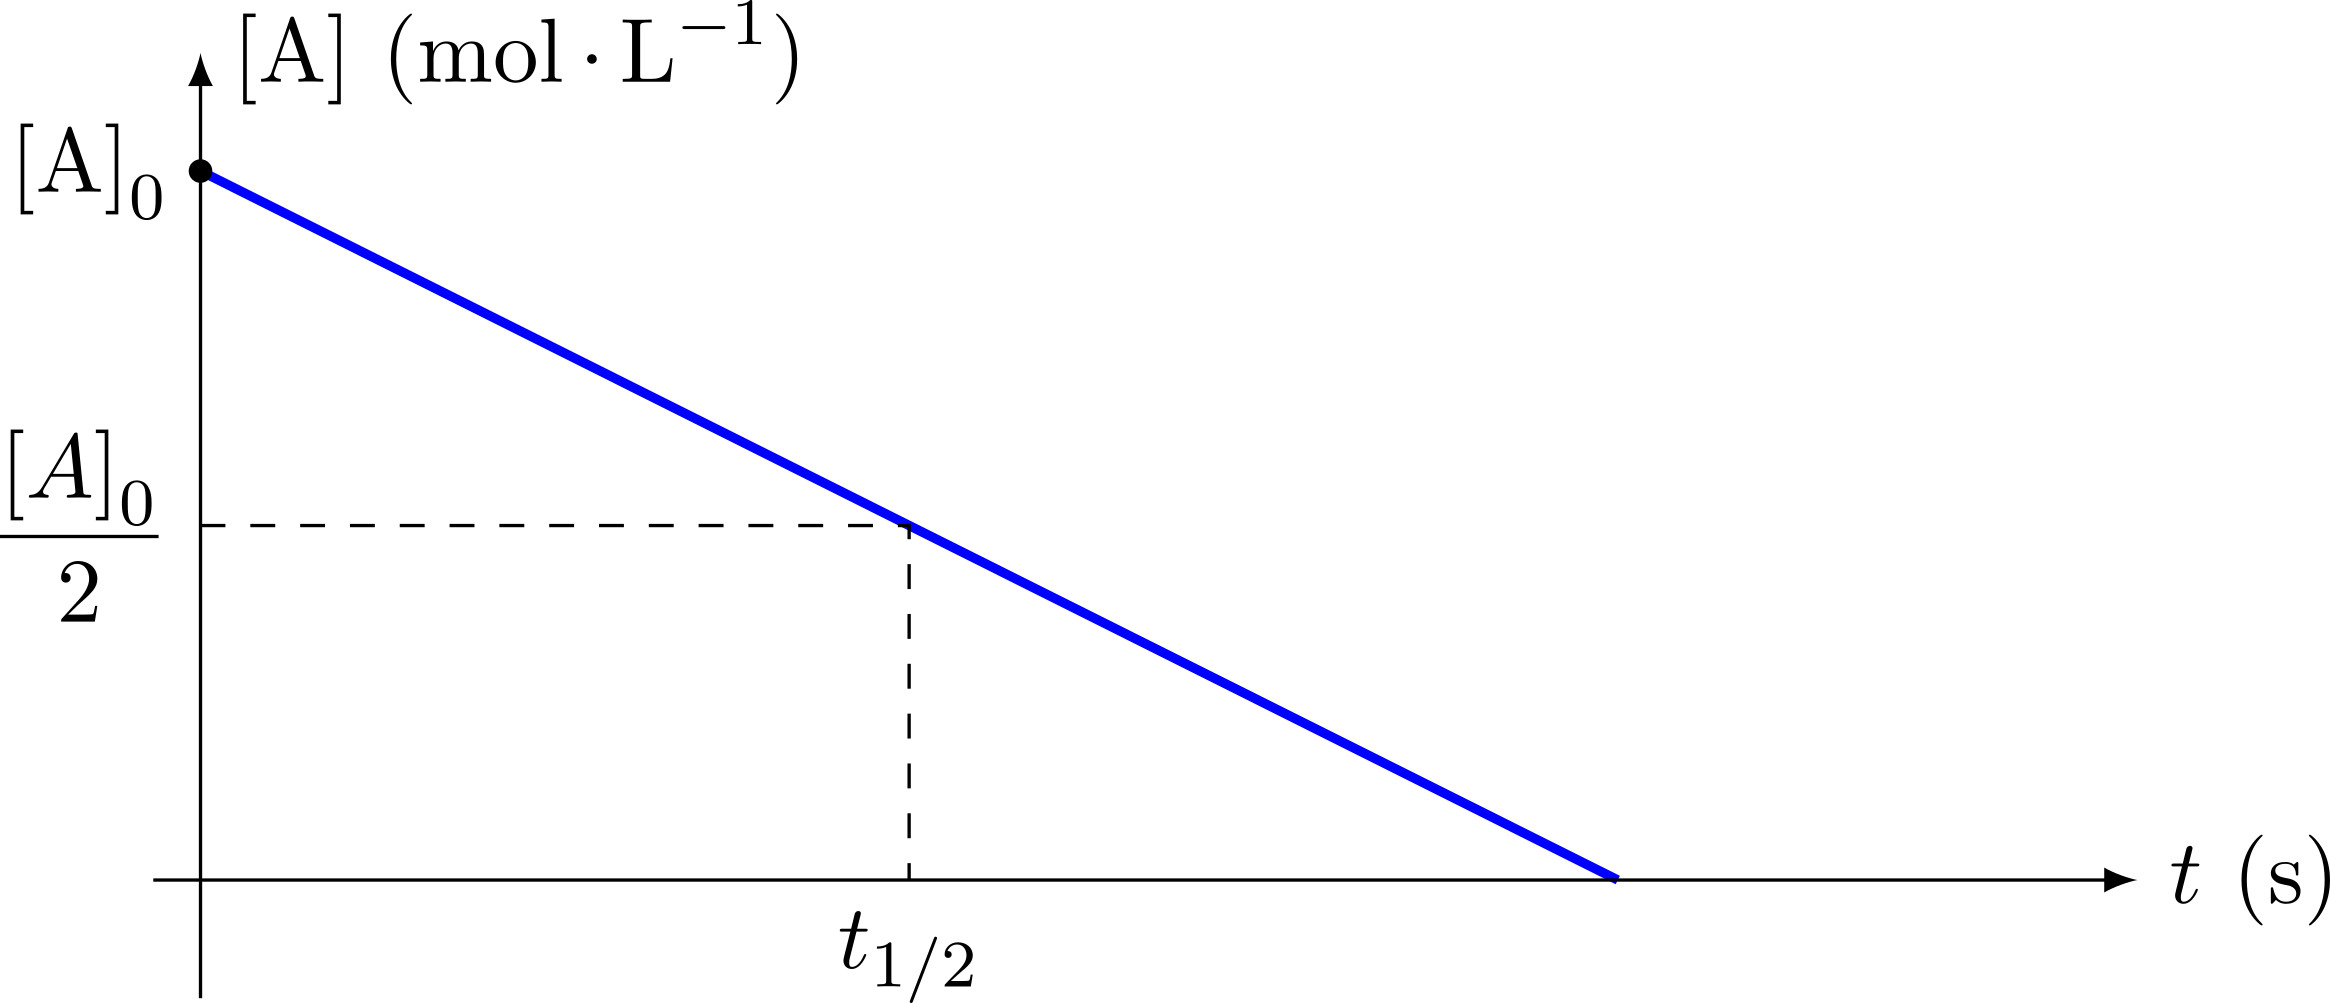
\includegraphics[width=.5\linewidth, draft=true]{ordre0}
	}{
		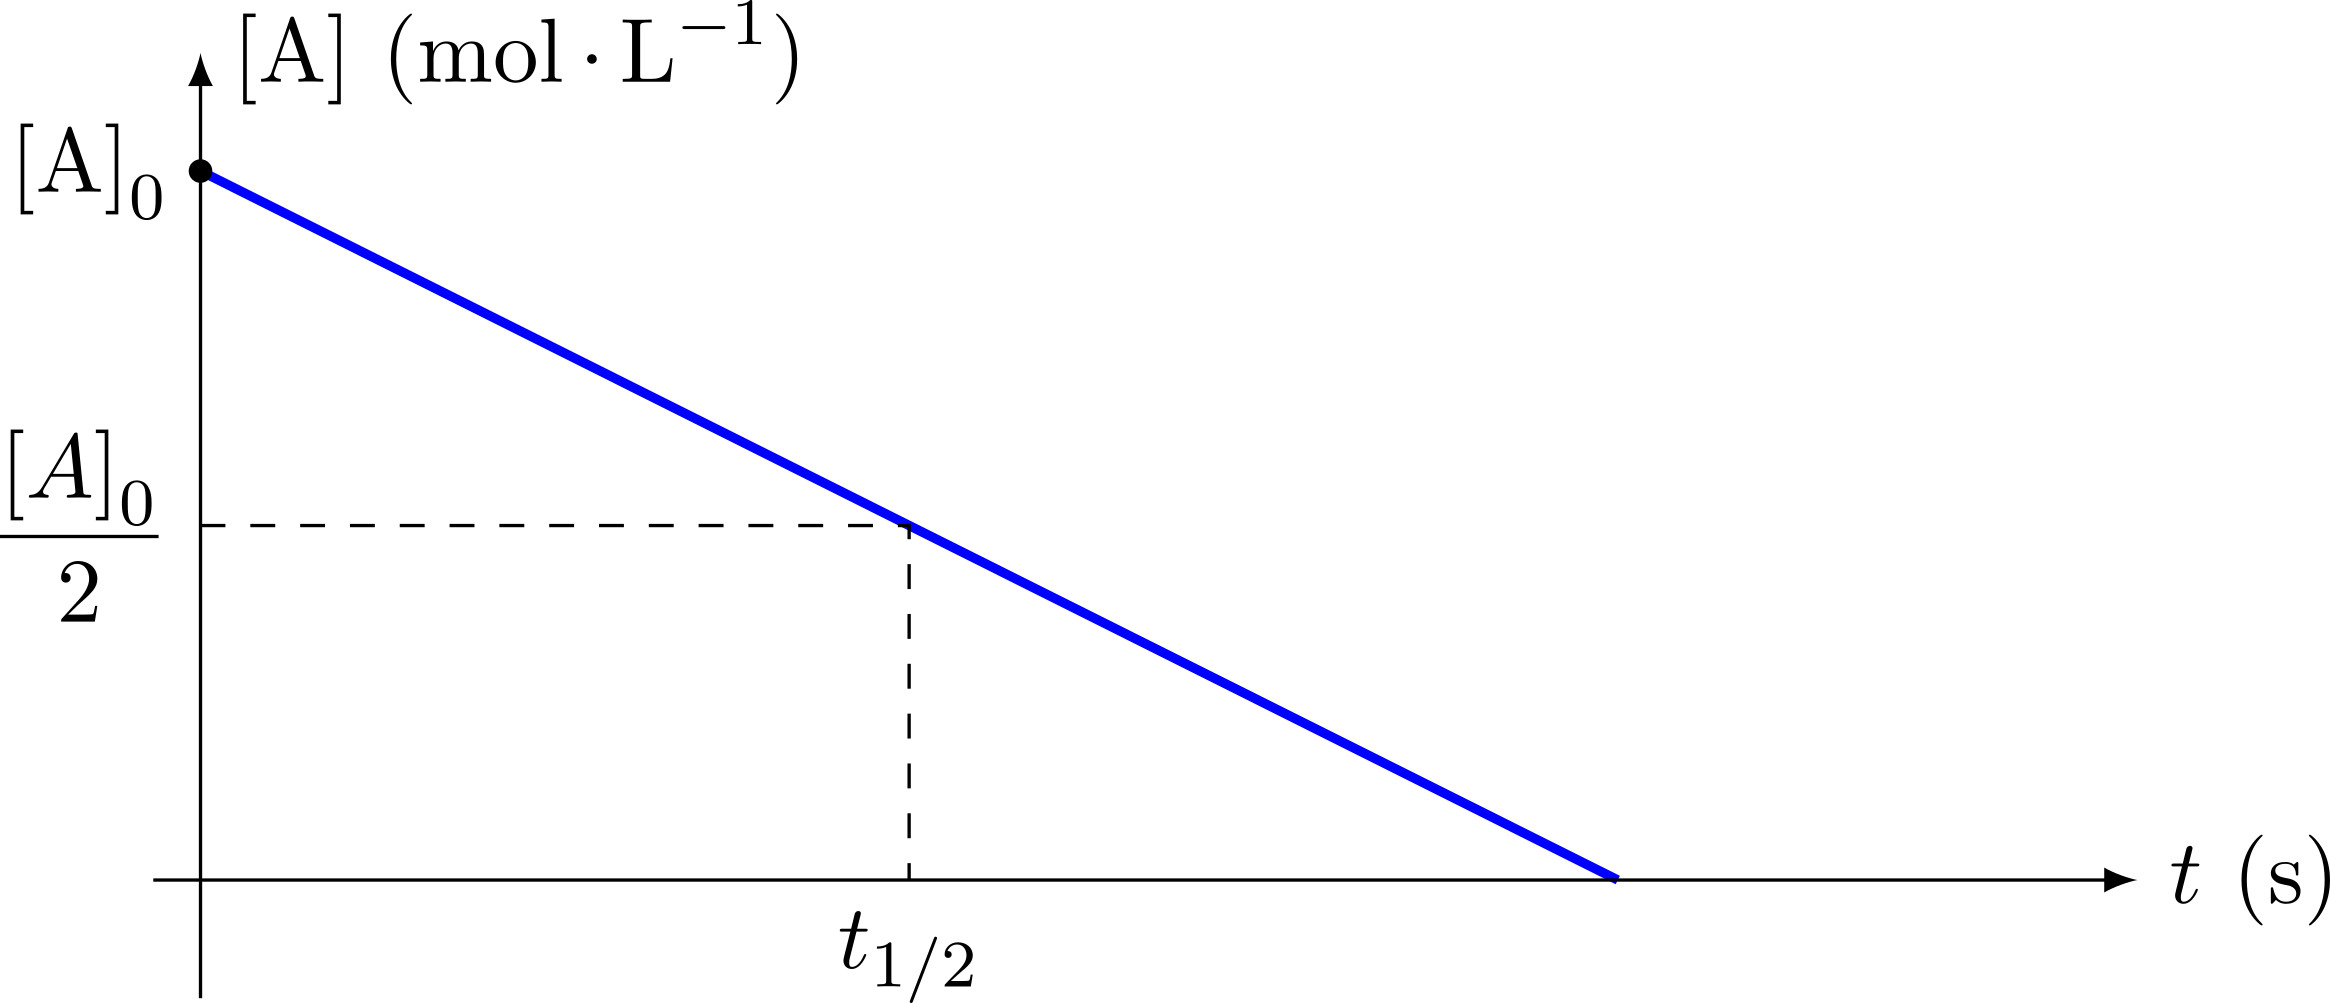
\includegraphics[width=.5\linewidth]{ordre0}
	}
	\captionof{figure}{Ordre 0}
\end{center}

\subsubsection{Temps de demi-réaction}
Dans le cas où A est le réactif limitant, et donc que sa concentration est nulle
à la fin de la réaction (comme sur le graphique), on a par définition
\psw{
	\begin{gather*}
		[{\ce{A}}](t_{1/2}) = \frac{[{\ce{A}}]_0}{2}
		\Lra
		[{\ce{A}}]_0 - kat_{1/2} = \frac{[{\ce{A}}]_0}{2}
		\\
		\Lra
		\boxed{t_{1/2} = \frac{[{\ce{A}}]_0}{2ka}}
	\end{gather*}
}

\subsubsection{Exemple}
La décomposition de l'alcool dans le sang suit une telle loi, avec une vitesse
$v \approx \SI{0.15}{g.L^{-1}.h^{-1}}$ selon l'individu.

\subsection{Ordre 1}

\subsubsection{Hypothèse}
\leftcenters{%
Soit la réaction
}{%
$
	a{\ce{A}} + b{\ce{B}}
	=
	c{\ce{C}} +d{\ce{D}}
$
}
\smallbreak
\leftcenters{%
	Avec la loi de vitesse
}{%
	\psw{
		$v = k [{\ce{A}}]$
	}
}

\subsubsection{Unité de $k$}

\psw{
	L'unité de $k$ \textbf{dans cette situation} est celle de $v$ divisée par celle
	d'une concentration~: c'est donc des $\si{s^{-1}}$.
}

\subsubsection{Équation différentielle}
On souhaite déterminer $[{\ce{A}}](t)$. Avec le lien entre vitesse de réaction et
vitesse de disparition, on a
\psw{
	\begin{gather*}
		\dv{[{\ce{A}}]}{t} = -av \Lra \dv{[{\ce{A}}]}{t} = -ka[{\ce{A}}]
		\\\Lra
		\boxed{\dv{[{\ce{A}}]}{t} + ka[{\ce{A}}] = 0}
	\end{gather*}
}

\subsubsection{Résolution}
La solution générale de cette équation du premier degré est
\psw{
	\[[{\ce{A}}](t) = K\exp(-kat)\]
}
avec $K$ une constante à déterminer par condition initiale. Ici, on a simplement
\psw{
	\begin{gather*}
		[{\ce{A}}](0) = [{\ce{A}}]_0 = K
		\\\Ra
		\boxed{[{\ce{A}}](t) = [{\ce{A}}]_0\exp(-kat)}
	\end{gather*}
	et la concentration diminue \textbf{exponentiellement avec le temps}. C'est le
	cas le plus fréquent.
}

\begin{center}
	\sswitch{
		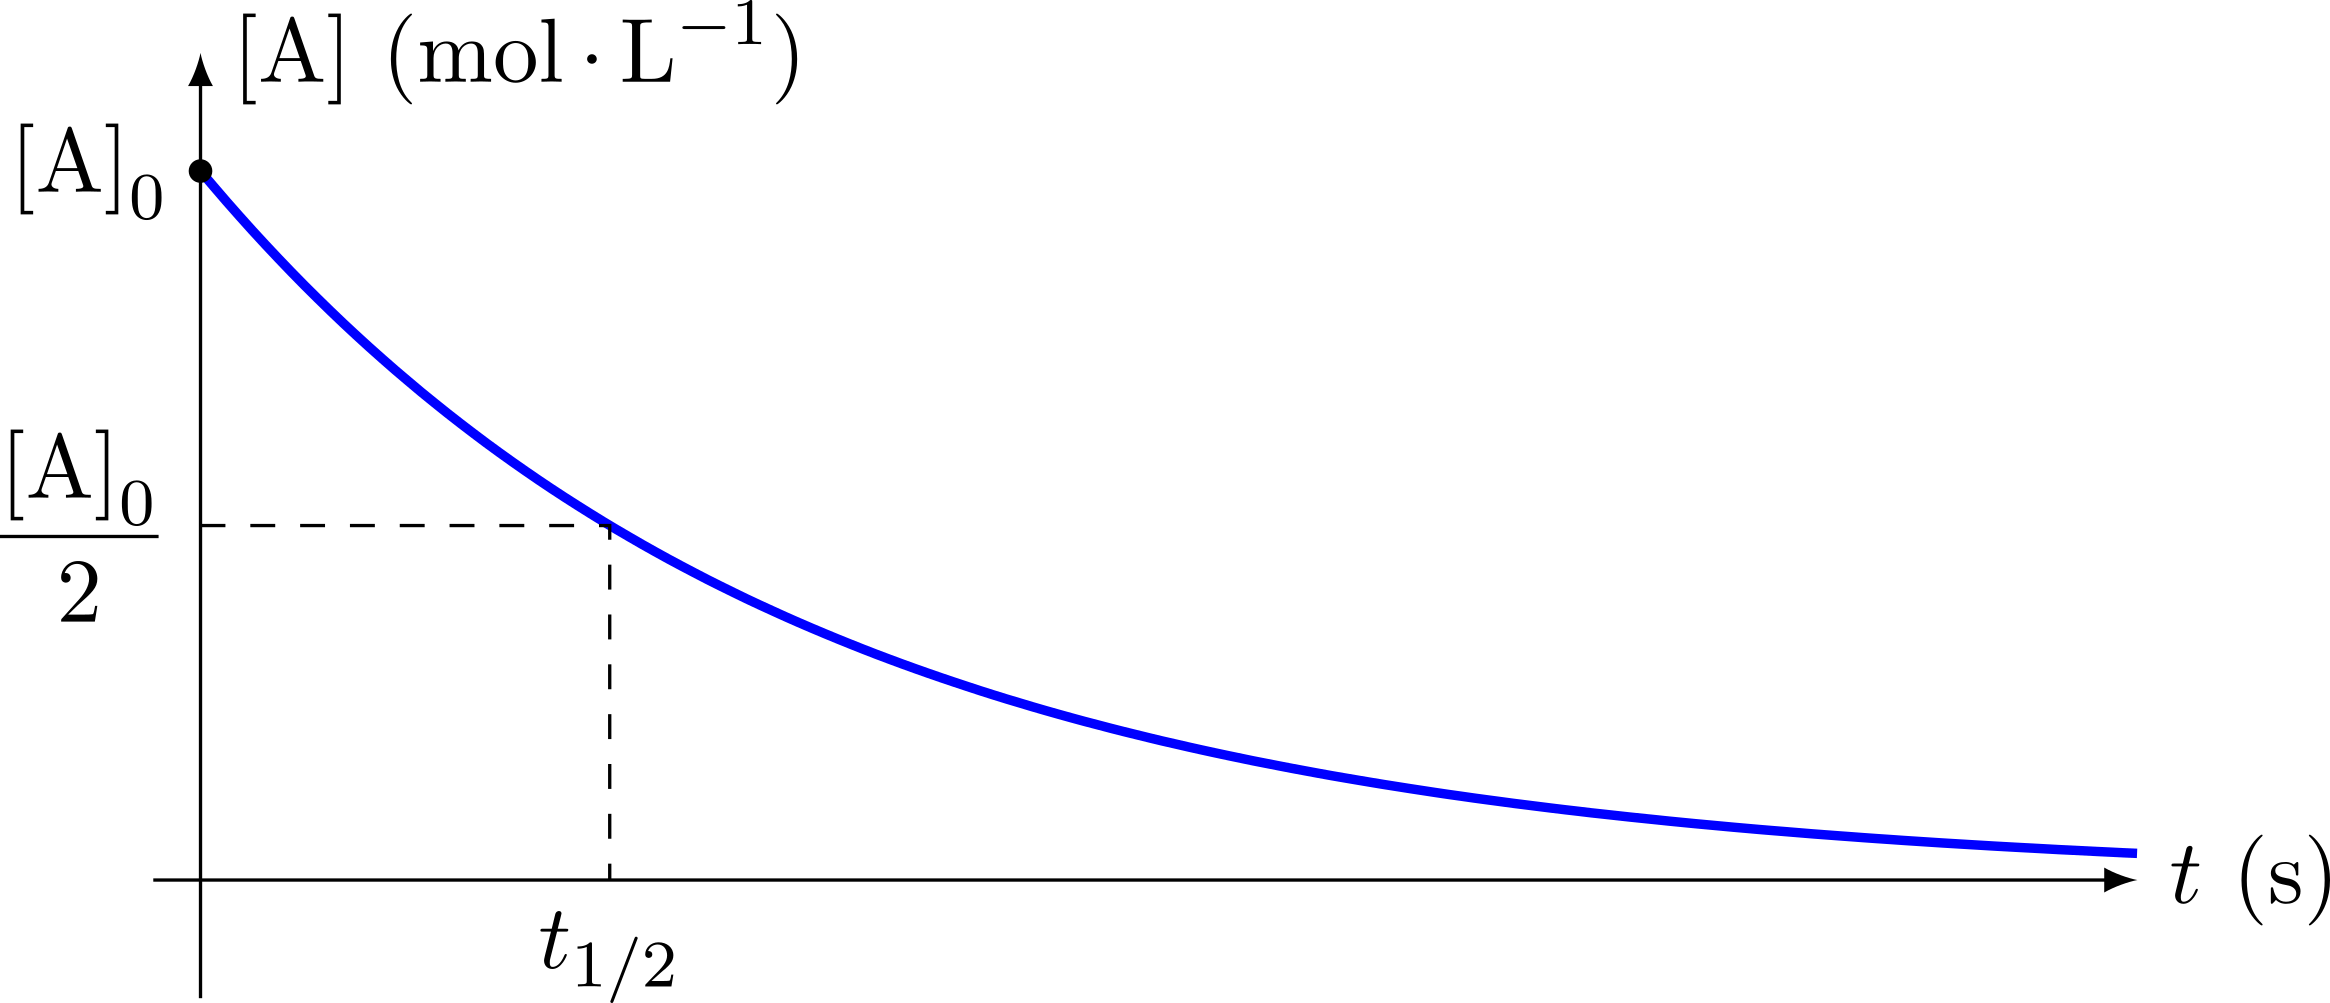
\includegraphics[width=.5\linewidth, draft=true]{ordre1}
	}{
		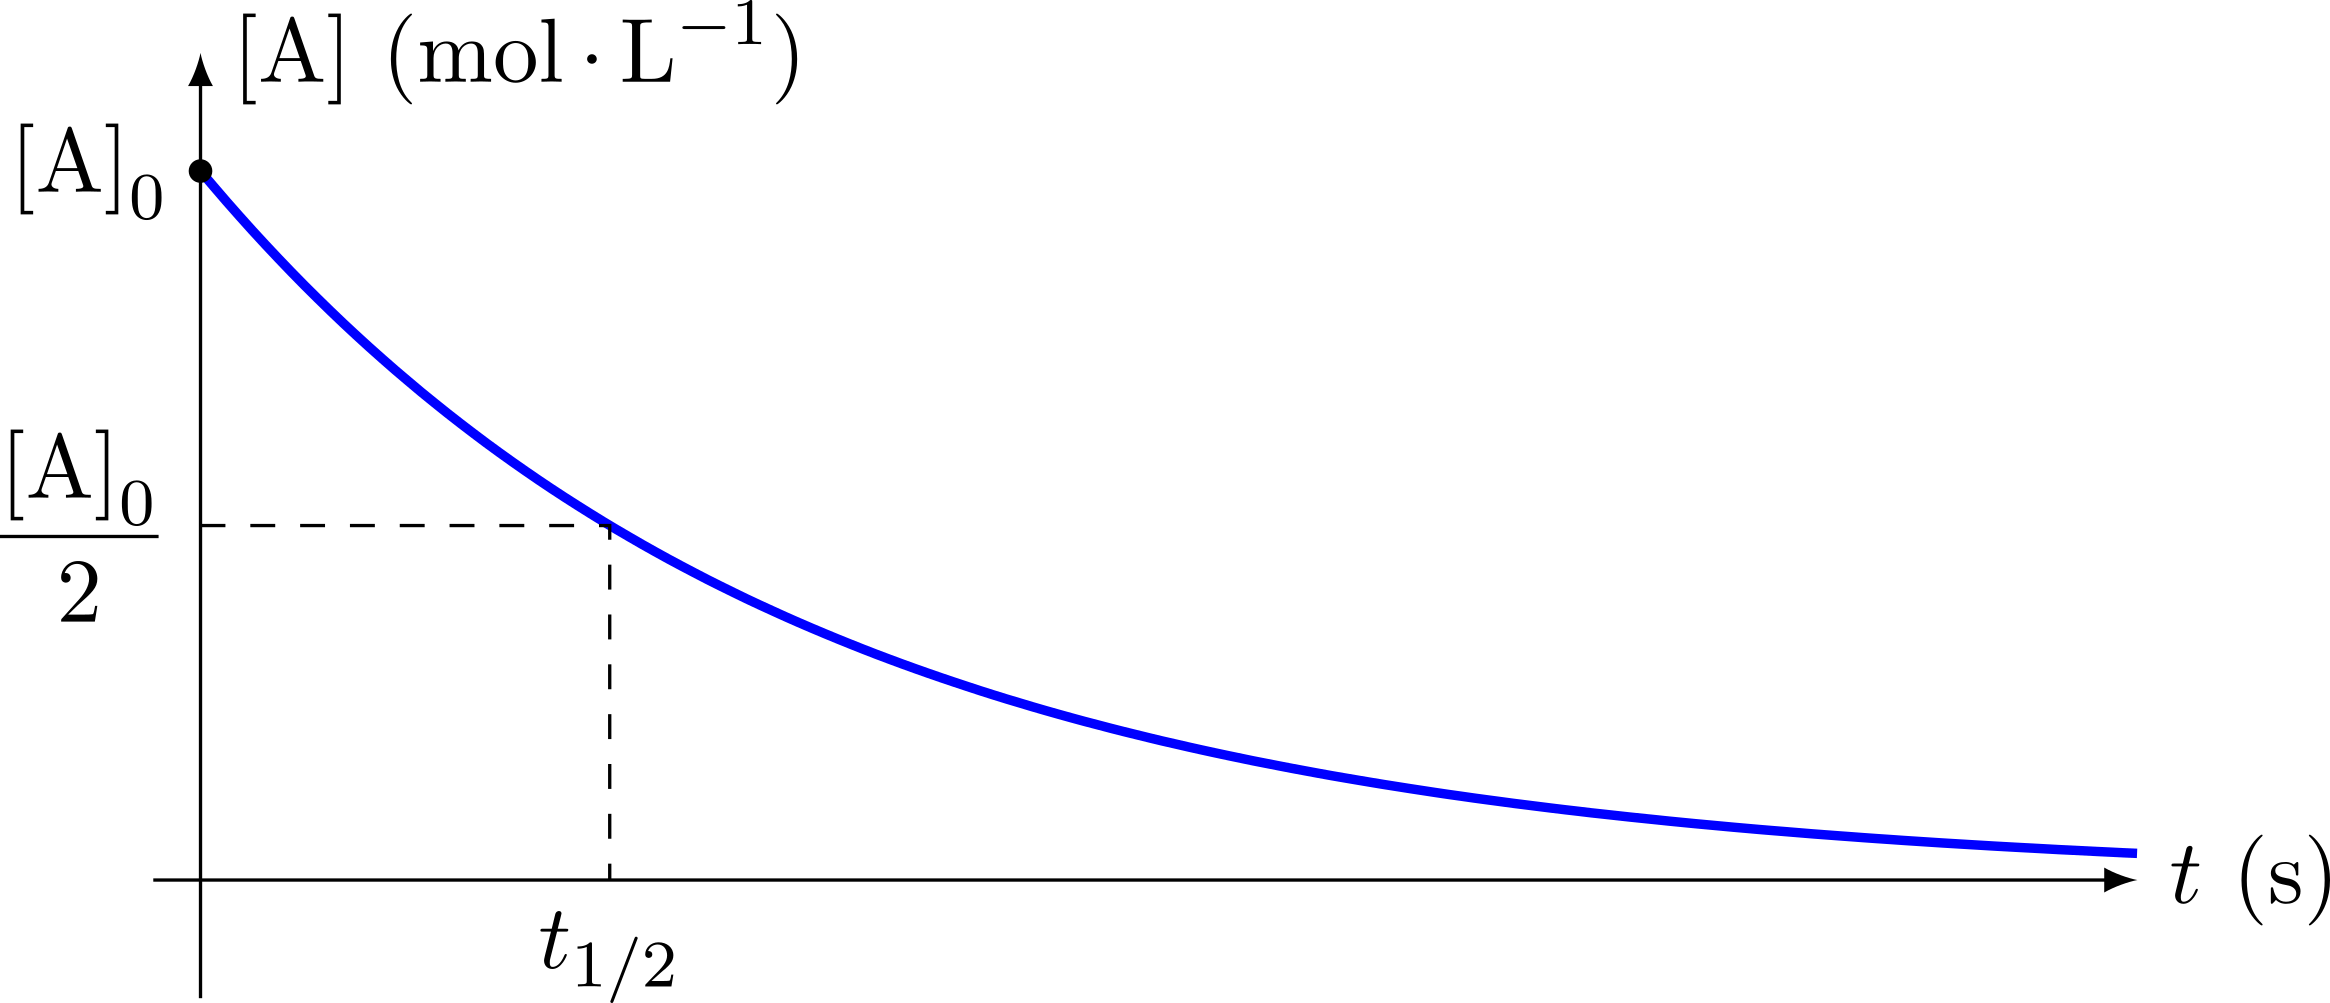
\includegraphics[width=.5\linewidth]{ordre1}
	}
	\captionof{figure}{Ordre 1}
\end{center}

\subsubsection{Temps de demi-réaction}
Dans le cas où A est le réactif limitant, et donc que sa concentration est nulle
à la fin de la réaction (comme sur le graphique), on a par définition
\psw{
	\begin{gather*}
		[{\ce{A}}](t_{1/2}) = \frac{[{\ce{A}}]_0}{2}
		\Lra
		[{\ce{A}}]_0\exp(-kat_{1/2}) = \frac{[{\ce{A}}]_0}{2}\\
		\Lra
		-kat_{1/2} = \ln \left( \frac{1}{2} \right) = -\ln 2\\
		\Lra
		\boxed{t_{1/2} = \frac{\ln 2}{ka}}
	\end{gather*}
}

\subsubsection{Exemple}
La désintégration du carbone 14 (et de tous les éléments radioactifs) suit une
cinétique d'ordre 1. Le principe de datation au carbone 14 est que pendant la
vie d'un organisme vivant, la proportion qu'il contient est égale à celle de
l'atmosphère par équilibre~: à sa mort, l'équilibre est rompu et le carbone se
désintègre. La demi-vie du ${\ce{^{14}C}}$ étant de
\SI{5730}{ans}, on peut mesurer la quantité de carbone 14 et donc l'âge d'un
échantillon jusqu'à environ \SI{50000}{ans}.

\subsection{Ordre 2}

\subsubsection{Hypothèse}
\leftcenters{%
Soit la réaction
}{%
$
	a{\ce{A}} + b{\ce{B}}
	=
	c{\ce{C}} +d{\ce{D}}
$
}
\smallbreak
\leftcenters{%
	Avec la loi de vitesse
}{%
	\psw{
		$v = k [{\ce{A}}]^2$
	}
}

\subsubsection{Unité de $k$}

\psw{
L'unité de $k$ \textbf{dans cette situation} est celle de $v$ divisée par une
concentration au carré~: c'est donc des $\si{mol^{-1}.L^.s^{-1}}$.
}

\subsubsection{Équation différentielle}
On souhaite déterminer $[{\ce{A}}](t)$. Avec le lien entre vitesse de réaction et
vitesse de disparition, on a
\psw{
\[
	\dv{[{\ce{A}}]}{t} = -av
	\Lra
	\boxed{\dv{[{\ce{A}}]}{t} = -ka[{\ce{A}}]^2}
\]
}

\subsubsection{Résolution}
C'est une équation différentielle \textbf{non-linéaire}. Il faut ruser pour la
résoudre. Pour cela, on \textbf{sépare les variables} et on utilise la dérivée de la
fonction inverse~: $\left( \frac{1}{f} \right)' = - \frac{f'}{f^2}$
\psw{
	\begin{DispWithArrows*}
		- \frac{\dd{[\ce{A}]}}{[{\ce{A}}]^2} &= ka \dd{t}
		\CArrow{$\int$}
		\\\Ra
		\frac{1}{[{\ce{A}}]} &= kat + K
	\end{DispWithArrows*}
}
avec $K$ une constante à déterminer par condition initiale. Ici, on a simplement
\psw{
	\[
		\frac{1}{[{\ce{A}}]_0} = K
		\qdonc
		\frac{1}{[{\ce{A}}]} = kat + \frac{1}{[{\ce{A}}]_0}
	\]
}
On a ainsi
\psw{
	\[
		\boxed{[{\ce{A}}](t) = \frac{1}{\frac{1}{[{\ce{A}}]_0} + kat}}
		\Lra
		\boxed{[{\ce{A}}](t) = \frac{[{\ce{A}}]_0}{1 + kat[{\ce{A}}]_0}}
	\]
}

\begin{center}
	\sswitch{
		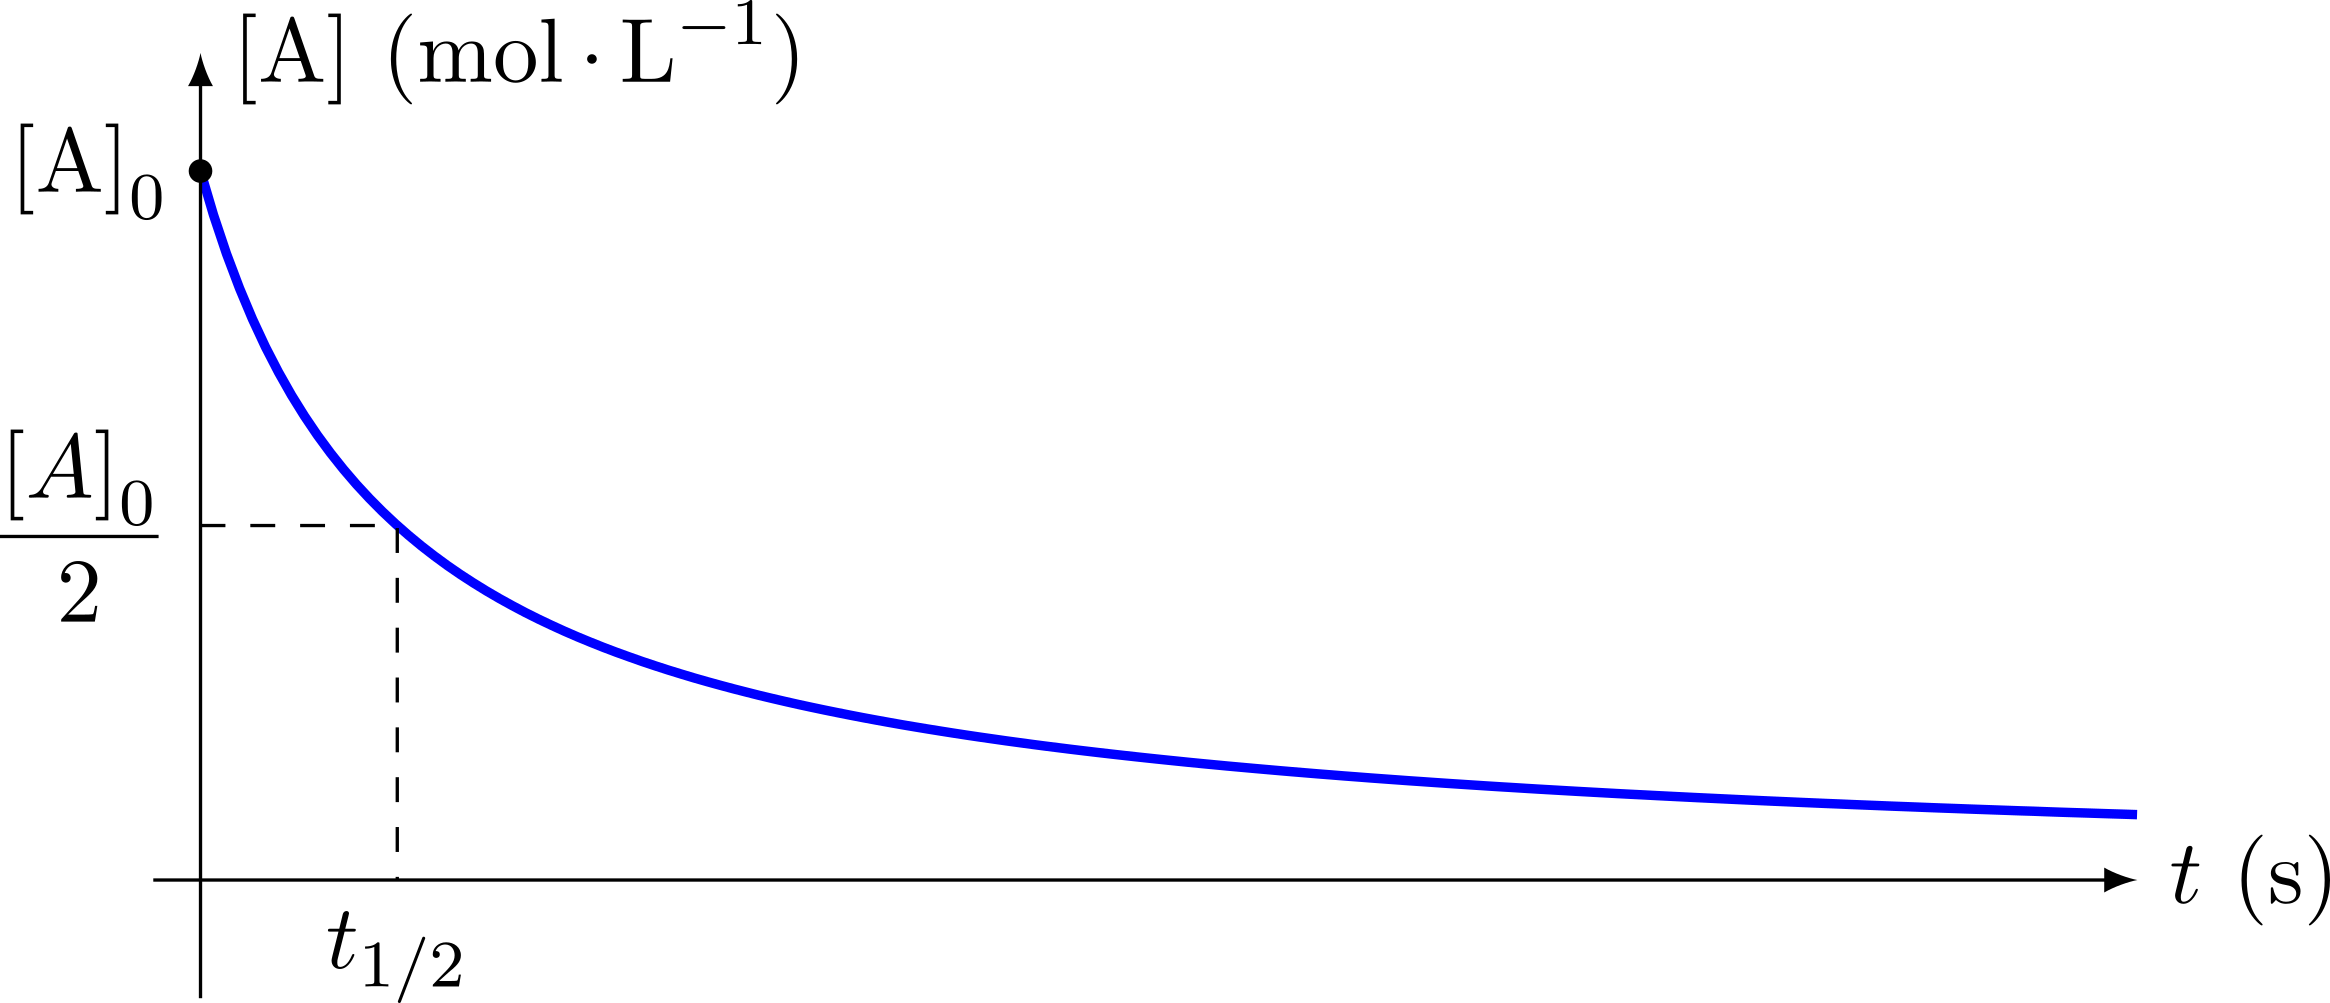
\includegraphics[width=.5\linewidth, draft=true]{ordre2}
	}{
		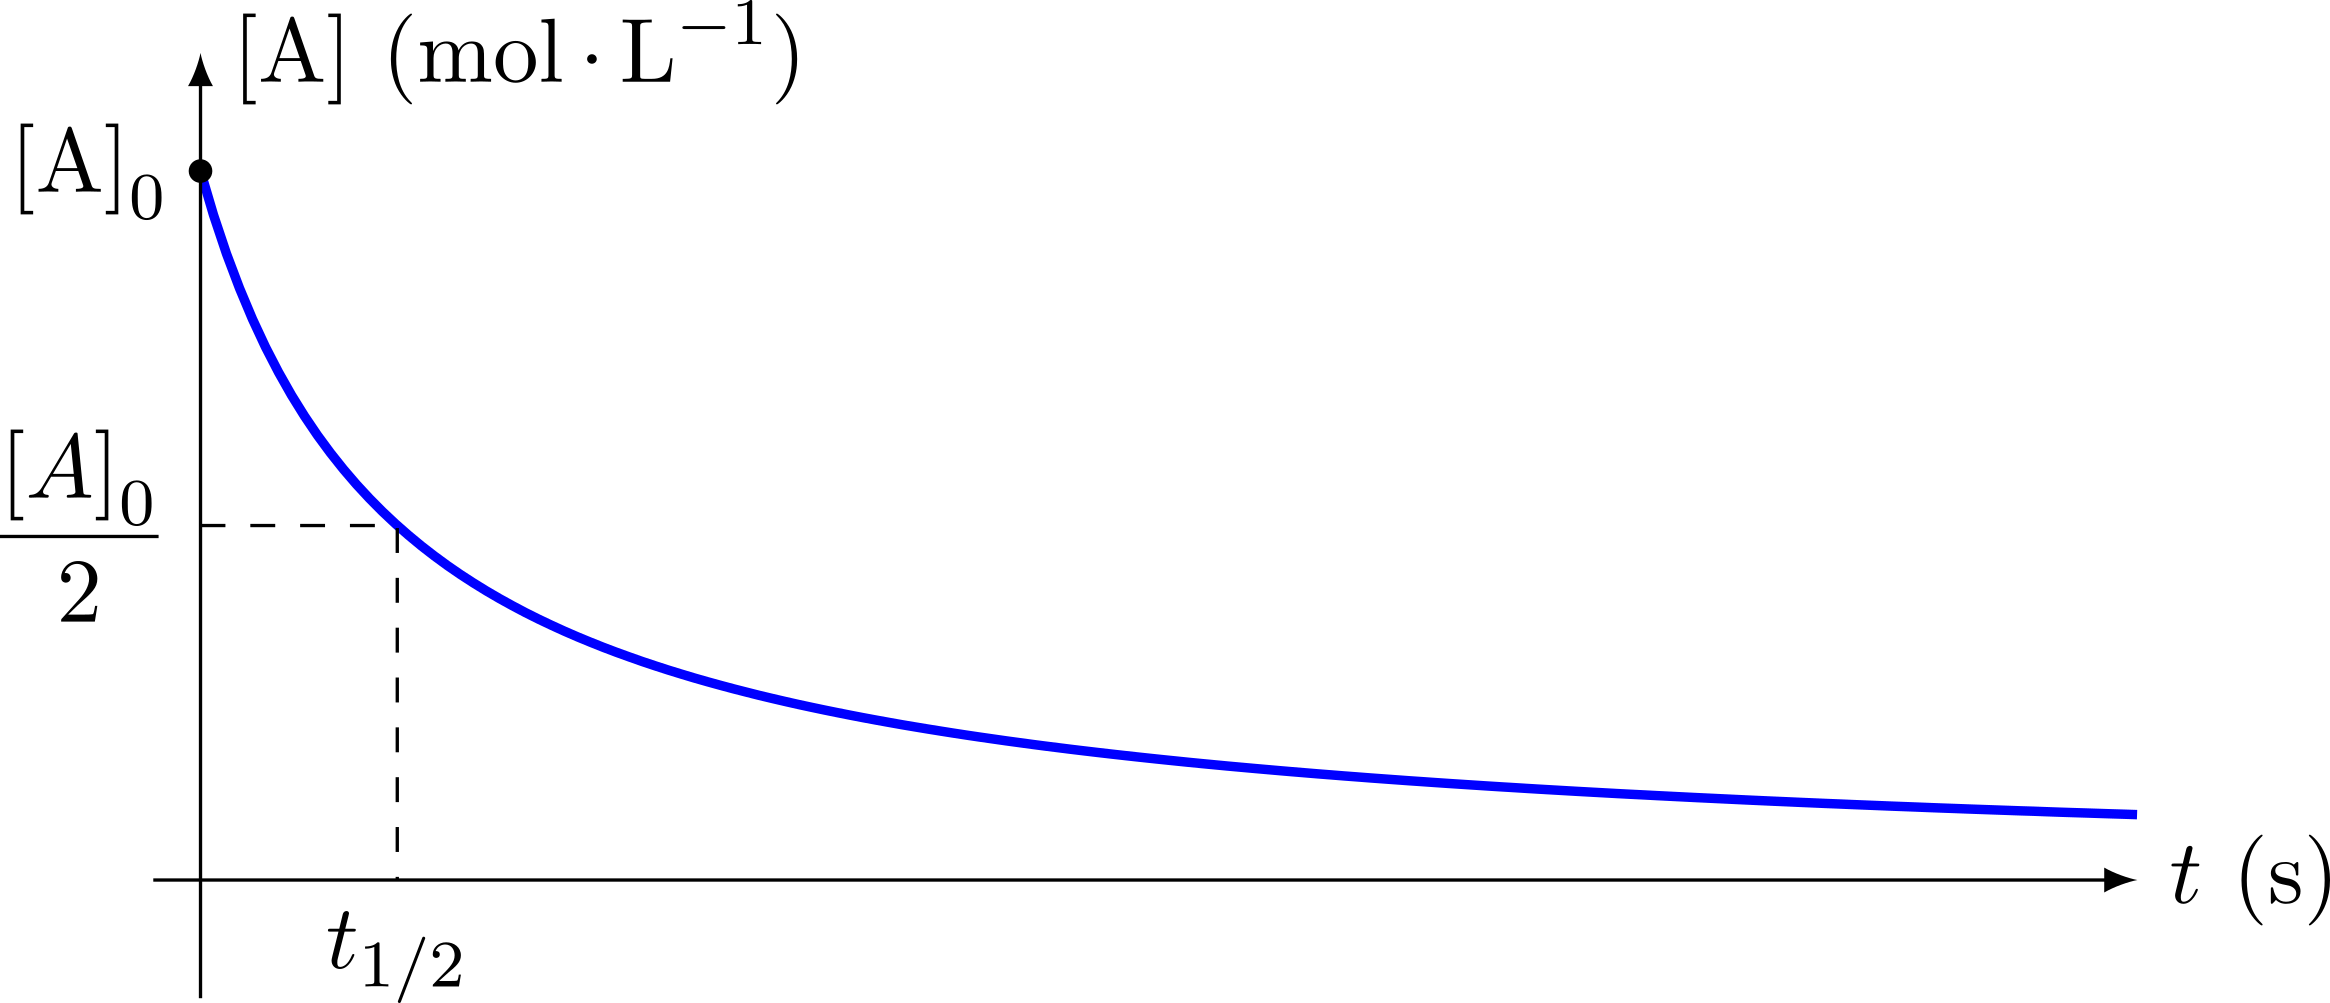
\includegraphics[width=.5\linewidth]{ordre2}
	}
	\captionof{figure}{Ordre 2}
\end{center}

\subsubsection{Temps de demi-réaction}
Dans le cas où A est le réactif limitant, et donc que sa concentration est nulle
à la fin de la réaction (comme sur le graphique), on a par définition
\psw{
	\begin{gather*}
		[{\ce{A}}](t_{1/2}) = \frac{[{\ce{A}}]_0}{2}
		\Lra
		\frac{[{\ce{A}}]_0}{1 + kat_{1/2}[{\ce{A}}]_0} = \frac{[{\ce{A}}]_0}{2}
		\\\Lra
		1 + kat_{1/2}[{\ce{A}}]_0 = 2
		\Lra
		\boxed{t_{1/2} = \frac{1}{ka[{\ce{A}}]_0}}
	\end{gather*}
}

\subsection{Expérimentalement}
\begin{itemize}
	\bitem{Méthode différentielle}~:
	\psw{
		on peut déterminer $v$ à partir de $[\ce{A}]$ et tracer $v$ en fonction de
		$[\ce{A}]$.
	}
	\bitem{Méthode intégrale}~:
	\psw{
		à partir de données expérimentales, on détermine l'ordre de la réaction en
		faisant un ajustement des données expérimentales par les solutions trouvées
		ci-dessus. On retient celle qui correspond le mieux aux données.
	}
	\bitem{Méthode de demi-réaction}~:
	\psw{
		le principe est de réaliser plusieurs expériences en modifiant
		$[\ce{A}]_0$. On relève à chaque fois le temps de demi-réaction (ou de
		façon plus générale un temps caractéristique).
	}
	\begin{itemize}
		\item \psw{
			      si $t_{1/2}$ est indépendant de $[\ce{A}]_0$, alors la cinétique
			      est d'ordre 1.
		      }
		\item \psw{
			      si $t_{1/2}$ est proportionnel à $[\ce{A}]_0$, alors la cinétique
			      est d'ordre 0.
		      }
		\item \psw{
			      si $t_{1/2}$ est inversement proportionnel à $[\ce{A}]_0$, alors
			      la cinétique est d'ordre 2.
		      }
	\end{itemize}
\end{itemize}

\subsection{Résumé}

\begin{tcb}[label=ror:resumeordre, tabularx={l|Y|Y|Y}](ror)
	{Différents ordres de réaction pour un unique réactif}
	&
	\textbf{Ordre 0 en A} &
	\textbf{Ordre 1 en A} &
	\textbf{Ordre 2 en A}
	\\\hline
	\rotatebox[origin=c]{90}{$v$, $[k]$} &
	\psw{
		\begin{center}
			$v = k$\\
			$k$ en $\si{mol.L^{-1}.s^{-1}}$
		\end{center}
	}
	&
	\psw{
		\begin{center}
			$v = k[{\ce{A}}]$\\
			$k$ en $\si{s^{-1}}$
		\end{center}
	}
	&
	\psw{
		\begin{center}
			$v = k[{\ce{A}}]^2$\\
			$k$ en $\si{mol^{-1}.L.s^{-1}}$
		\end{center}
	}
	\\\hline
	\rotatebox[origin=c]{90}{ED} &
	\psw{\[\dv{[{\ce{A}}]}{t} + ka = 0\]}
	&
	\psw{\[\dv{[{\ce{A}}]}{t} + ka [{\ce{A}}] = 0\]}
	&
	\psw{\[\dv{[{\ce{A}}]}{t} + ka [{\ce{A}}]^2 = 0\]}
	\\\hline
	\rotatebox[origin=c]{90}{Solution} &
	\psw{\[\boxed{[{\ce{A}}](t) = [{\ce{A}}]_0 - kat}\]}
	&
	\psw{\[\boxed{[{\ce{A}}](t) = [{\ce{A}}]_0\exp(-kat)}\]}
	&
	\psw{\[\boxed{[{\ce{A}}](t) = \frac{[{\ce{A}}]_0}{1 + kat[{\ce{A}}]_0}}\]}
	\\\hline
	\rotatebox[origin=c]{90}{$t_{1/2}$} &
	\psw{\[t_{1/2} = \frac{[{\ce{A}}]_0}{2ka}\]}
	&
	\psw{\[t_{1/2} = \frac{\ln 2}{ka}\]}
	&
	\psw{\[t_{1/2} = \frac{1}{ka[{\ce{A}}]_0}\]}
	\\\hline
	\rotatebox[origin=c]{90}{Graphiques} &
	\begin{center}
		\sswitch{
			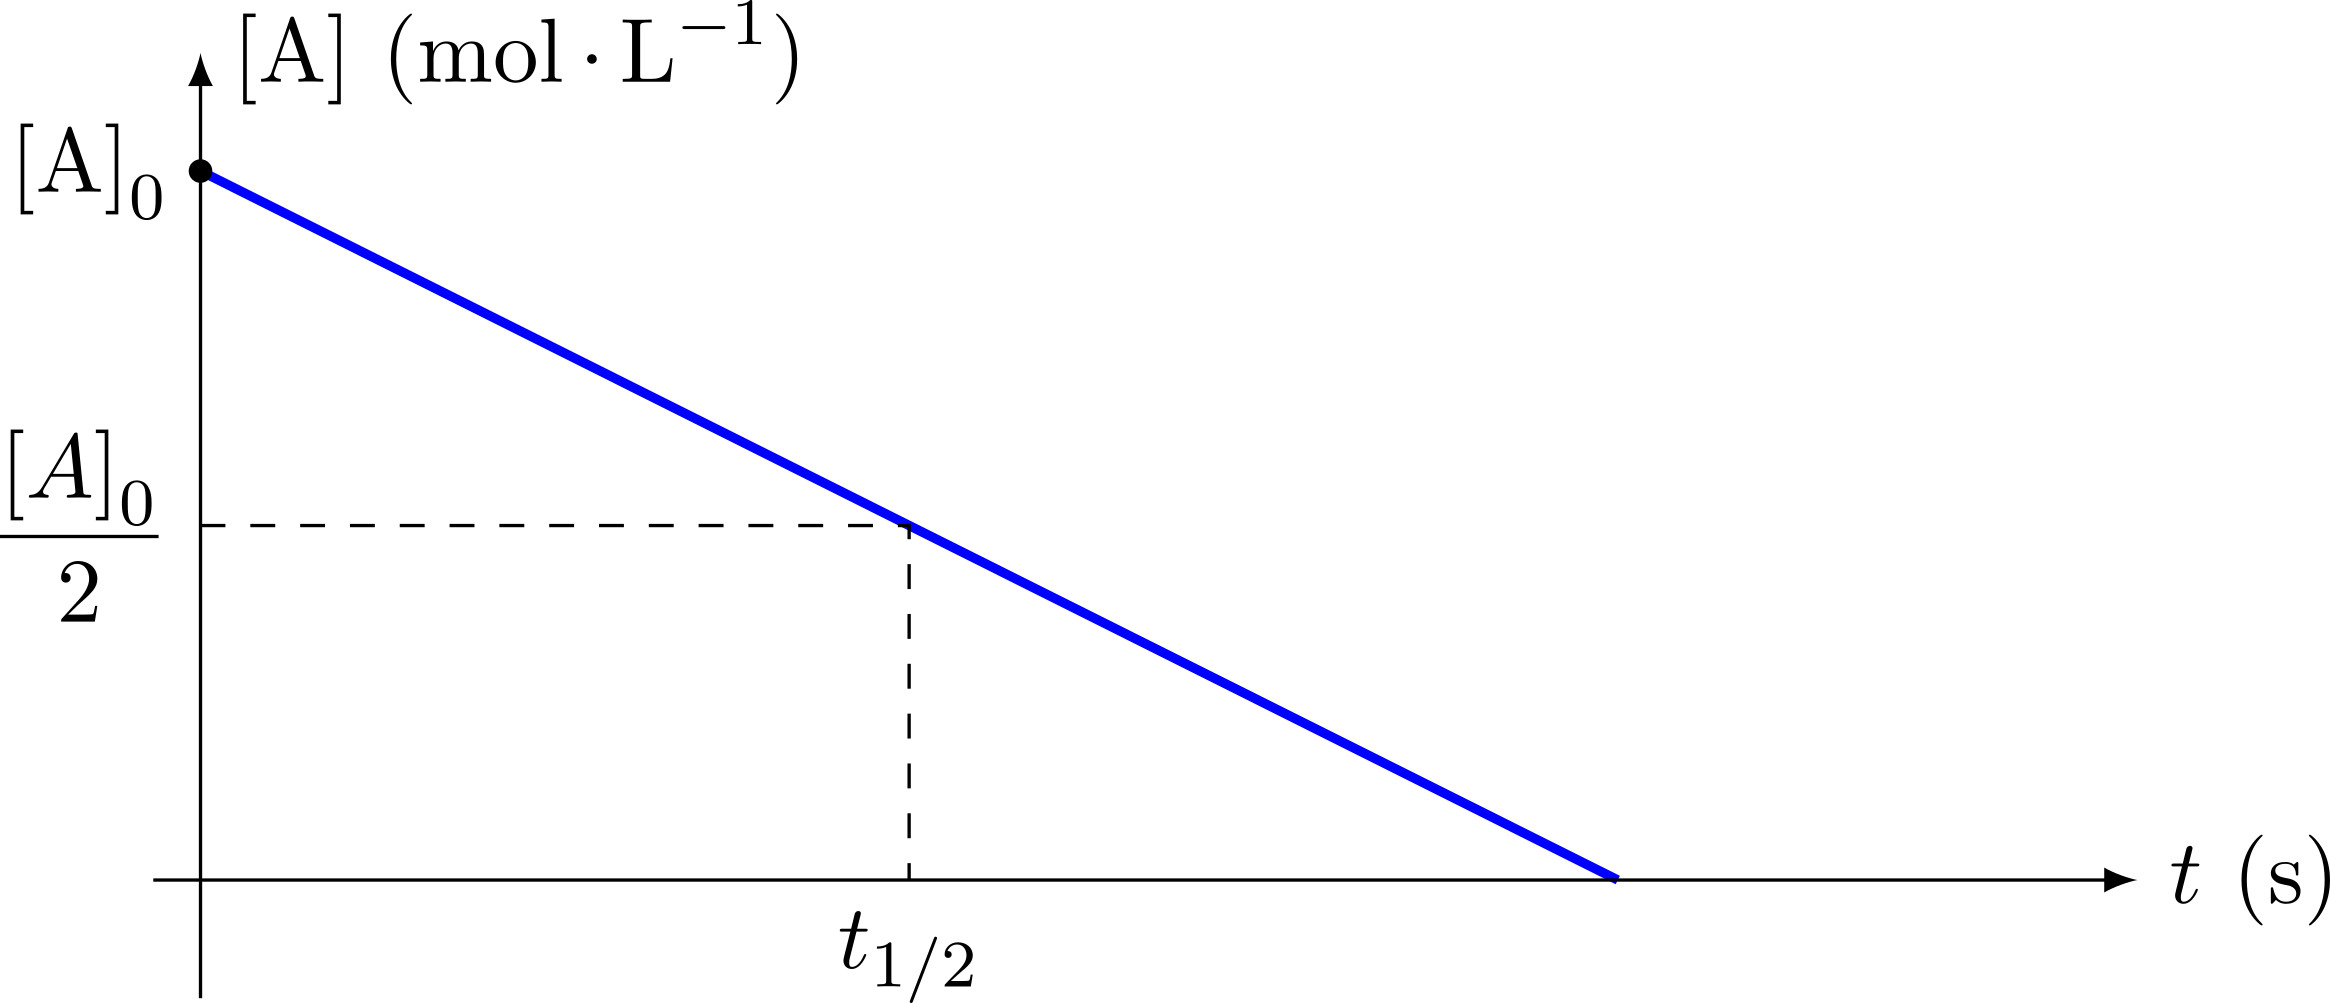
\includegraphics[width=\linewidth, draft=true]{ordre0}
		}{
			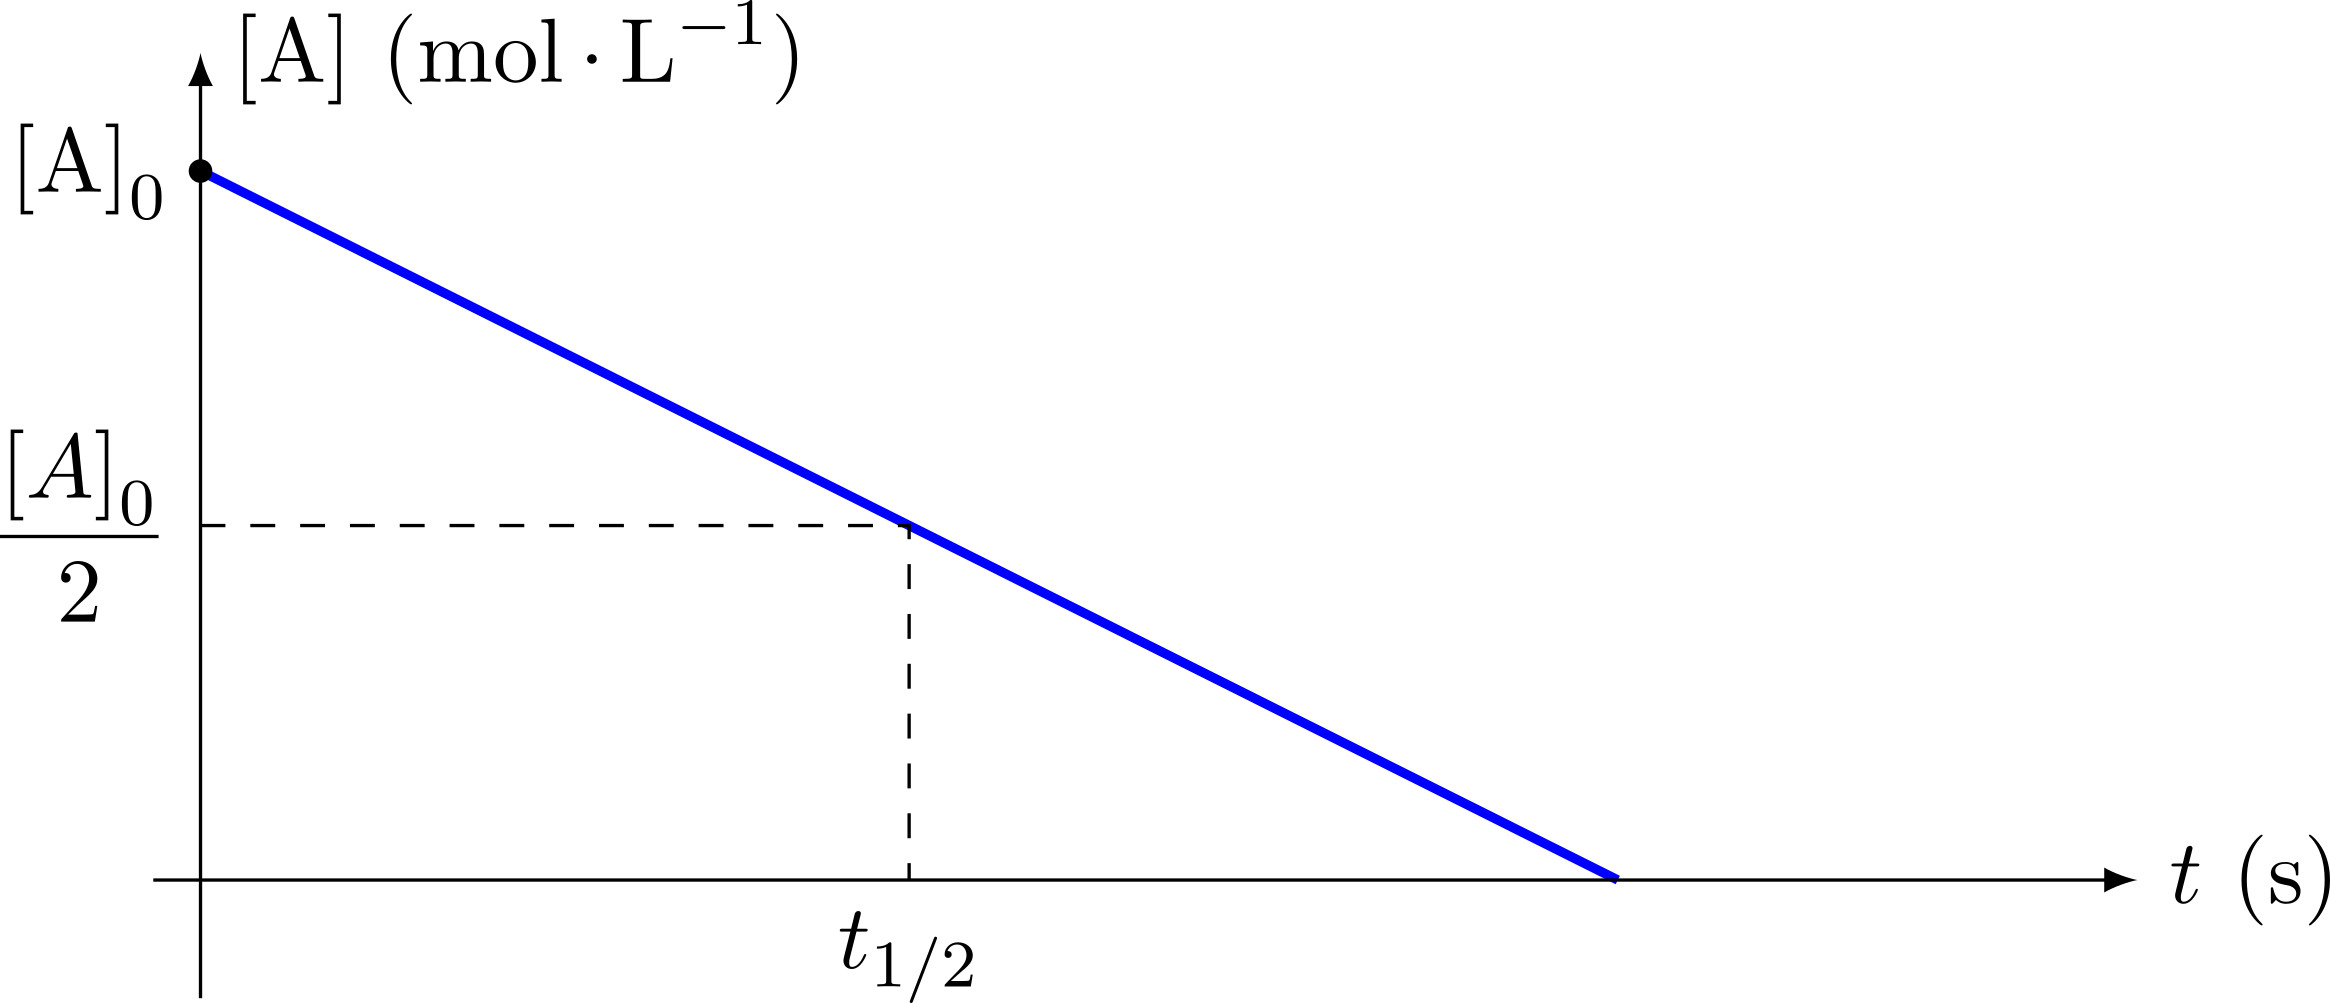
\includegraphics[width=\linewidth]{ordre0}
		}
		\captionof{figure}{Ordre 0}
	\end{center}
	&
	\begin{center}
		\sswitch{
			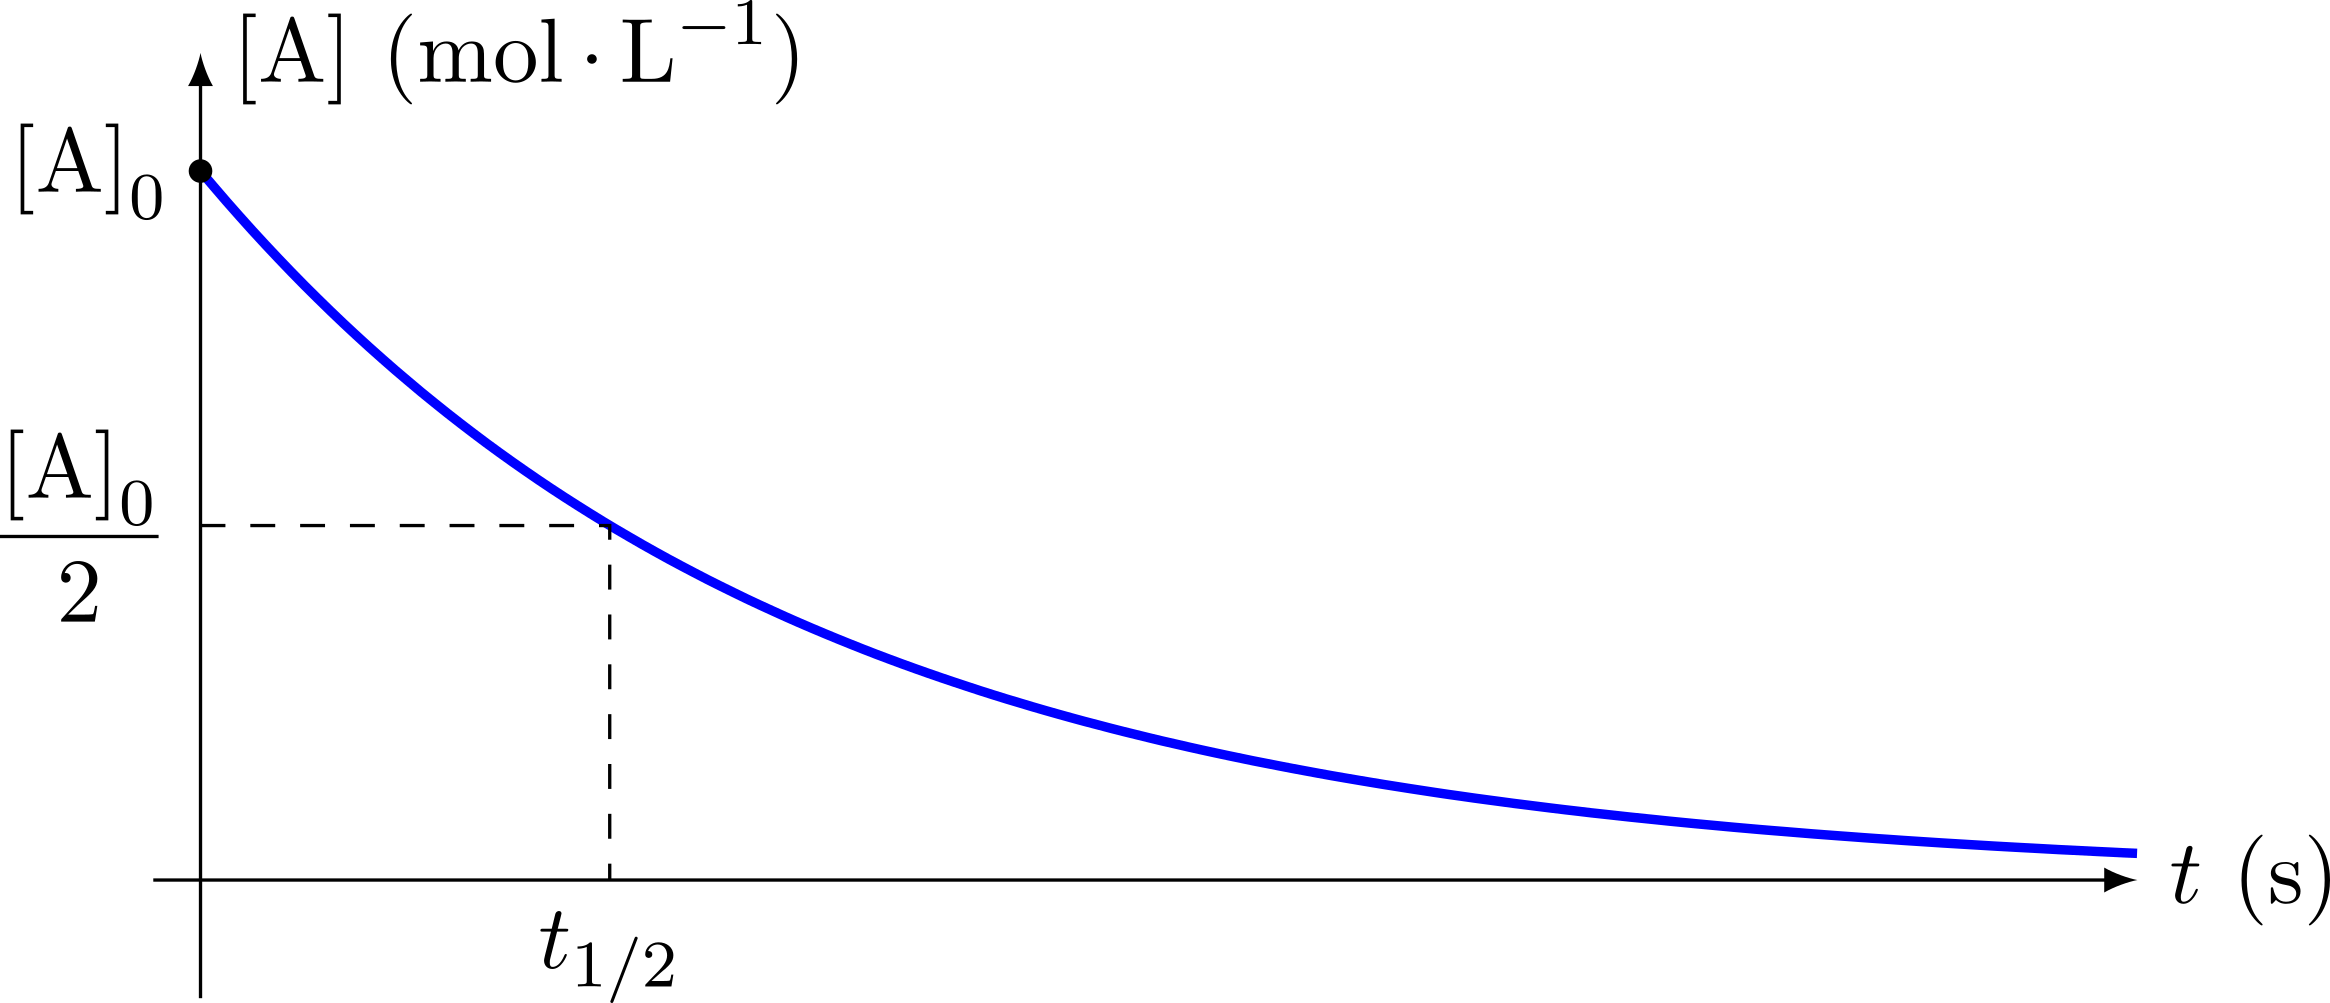
\includegraphics[width=\linewidth, draft=true]{ordre1}
		}{
			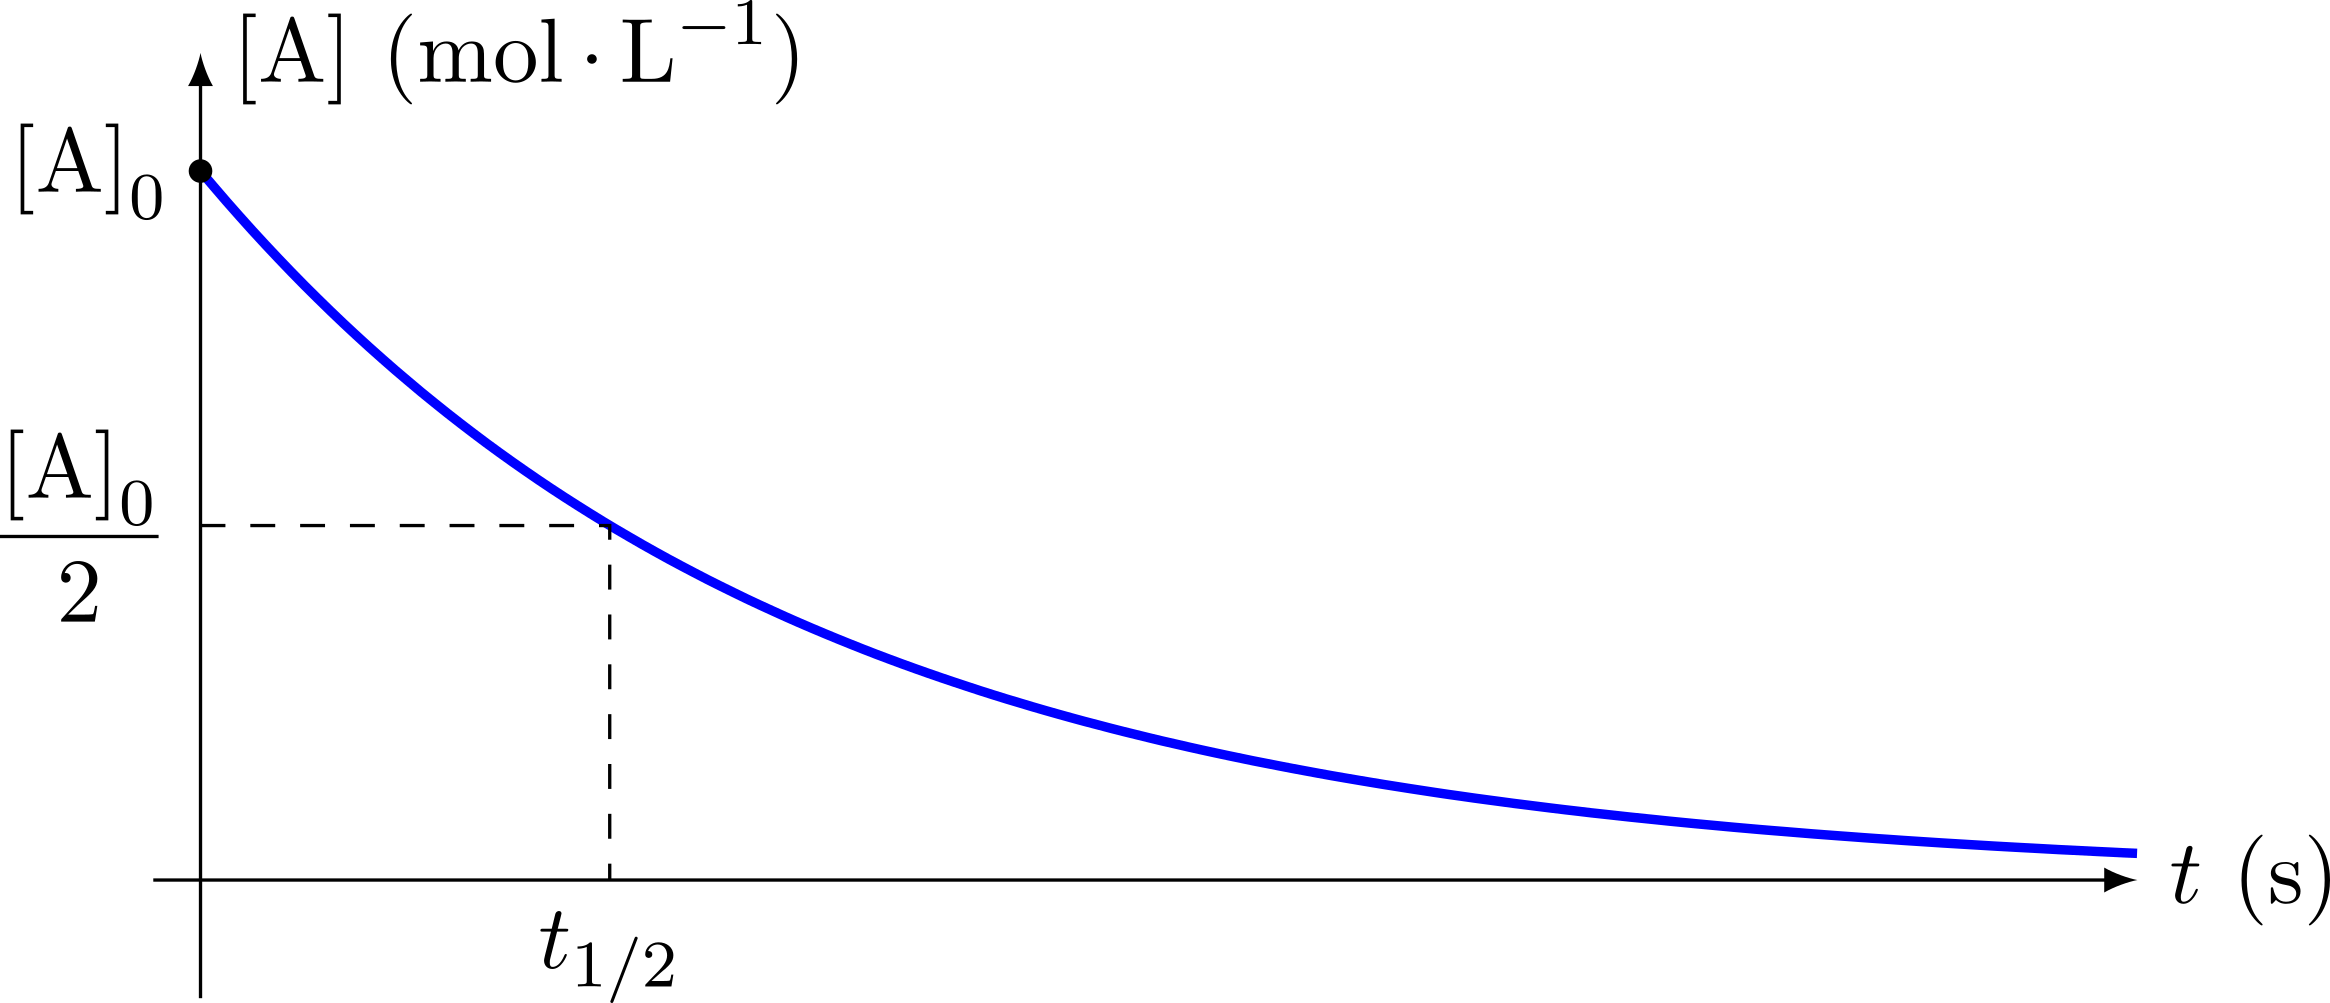
\includegraphics[width=\linewidth]{ordre1}
		}
		\captionof{figure}{Ordre 1}
	\end{center}
	&
	\begin{center}
		\sswitch{
			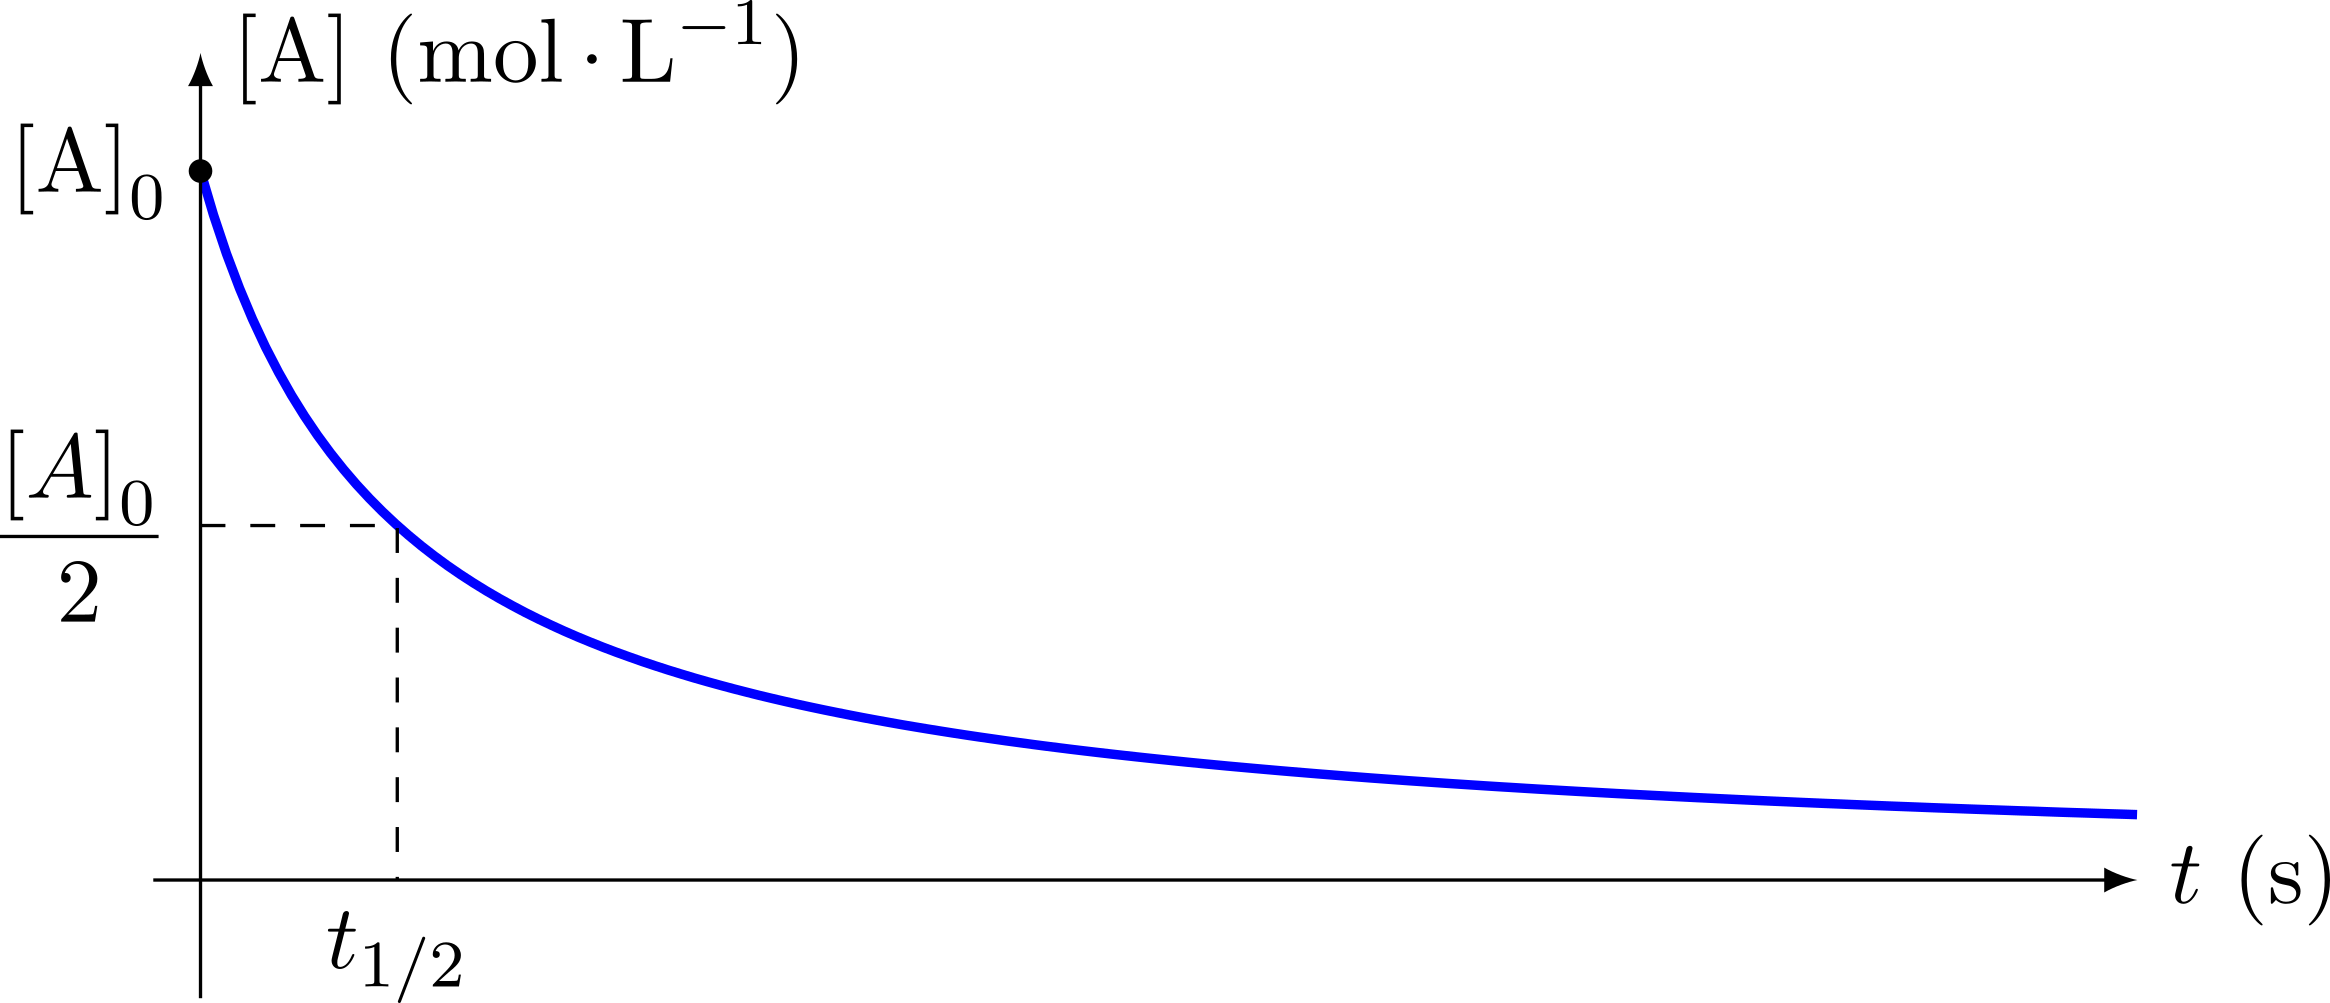
\includegraphics[width=\linewidth, draft=true]{ordre2}
		}{
			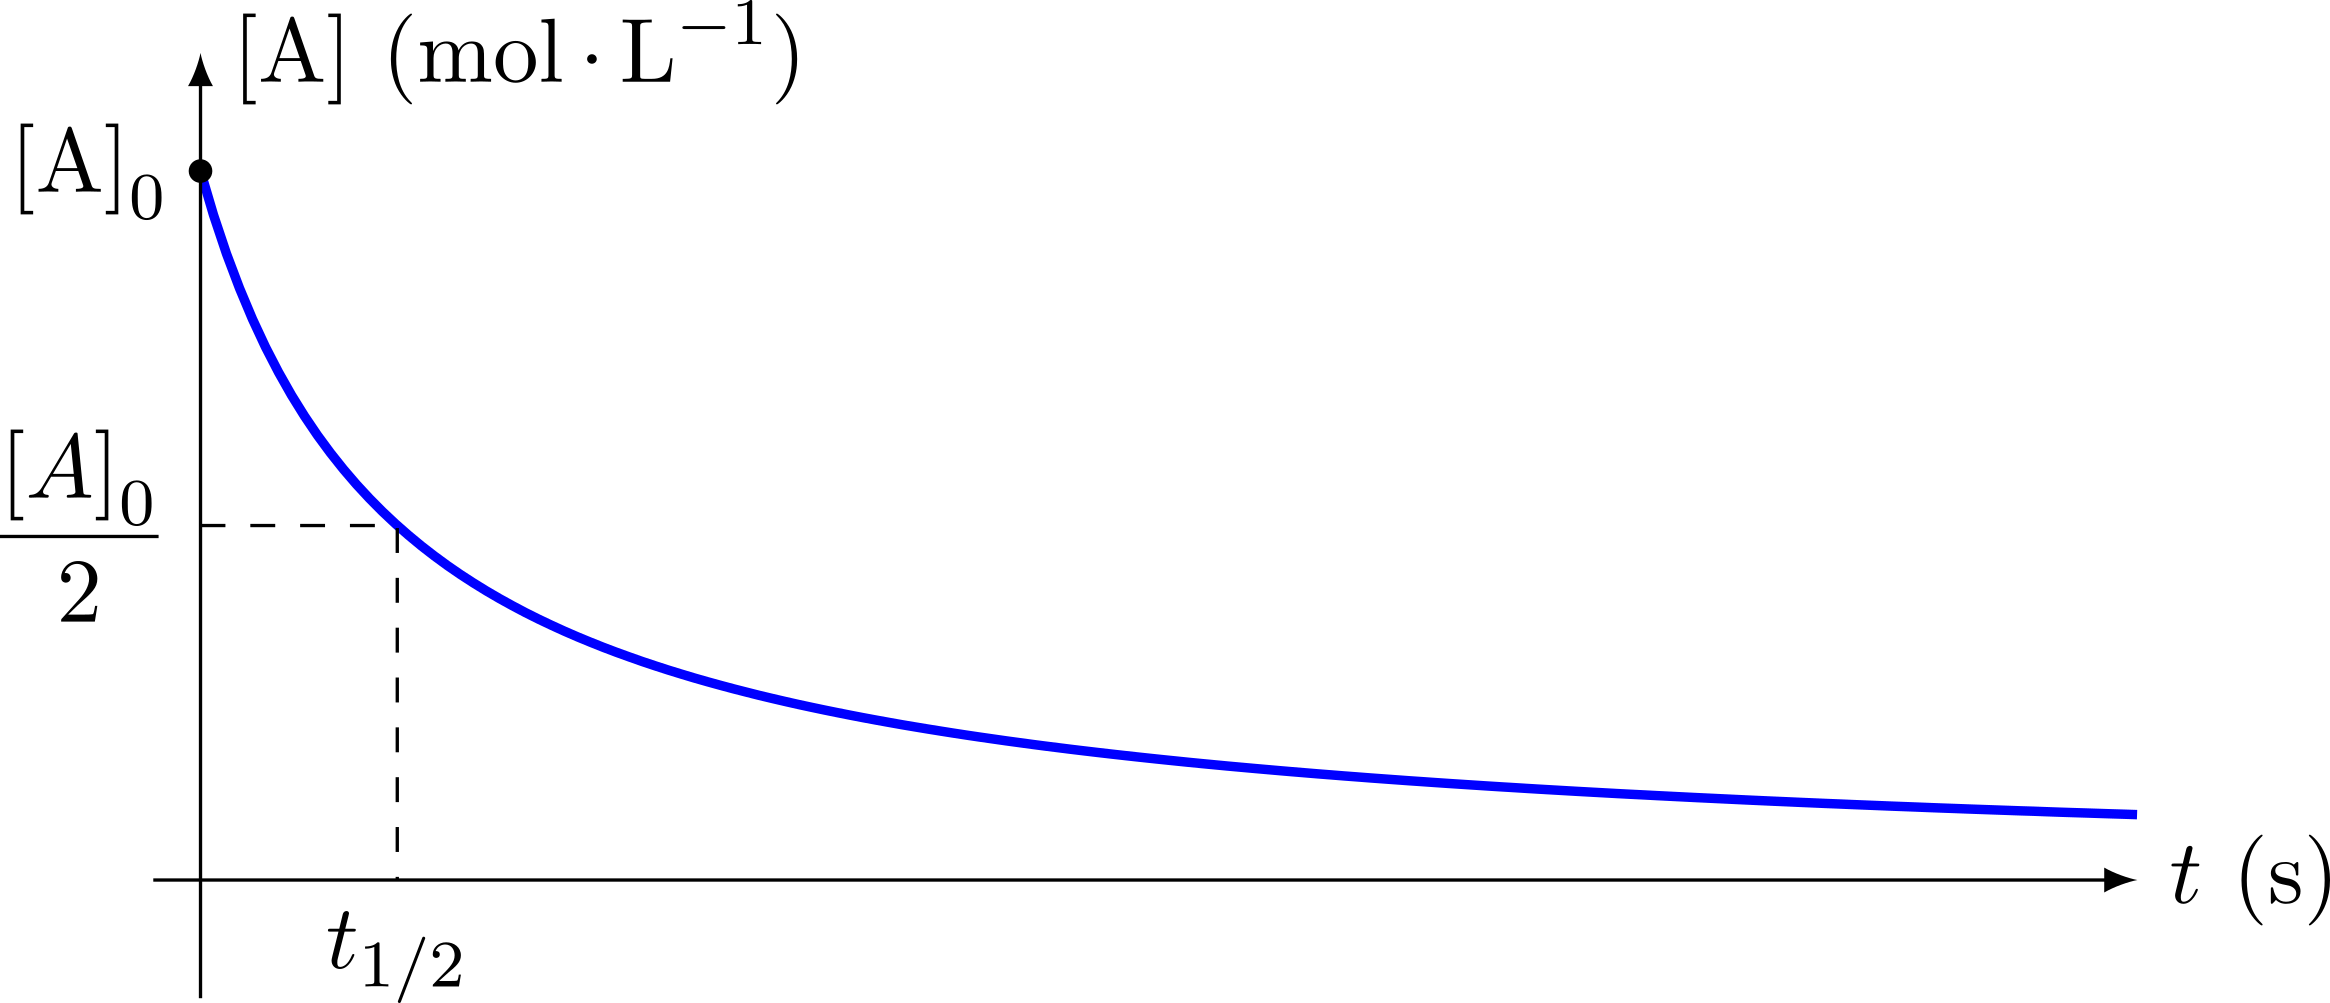
\includegraphics[width=\linewidth]{ordre2}
		}
		\captionof{figure}{Ordre 2}
	\end{center}
\end{tcb}

\begin{tcb}*(expe)<itc>"trans"{Transition}
	Après avoir vu l'impact de la concentration sur la vitesse, regardons
	comment quantifier l'impact de la température sur la vitesse.
\end{tcb}

\vspace{-15pt}
\section{Température et loi d'\textsc{Arrhénius}}
\subsection{Phénoménologie}
Comme nous l'avons vu au début du chapitre, la température augmente la vitesse
de réaction, ce que nous avons traduit par l'idée de choc efficace.

En effet, dans le milieu réactionnel, les molécules ont une distribution de
vitesse répartie autour d'une valeur moyenne, $v^*$, comme présenté ci-dessous à
gauche~; celles qui ont la plus grande vitesse et donc énergie cinétique ont la
capacité de passer la barrière de potentielle nécessaire à la réaction,
représentée ci-dessous à droite.

\begin{minipage}{0.49\linewidth}
	\sswitch{
		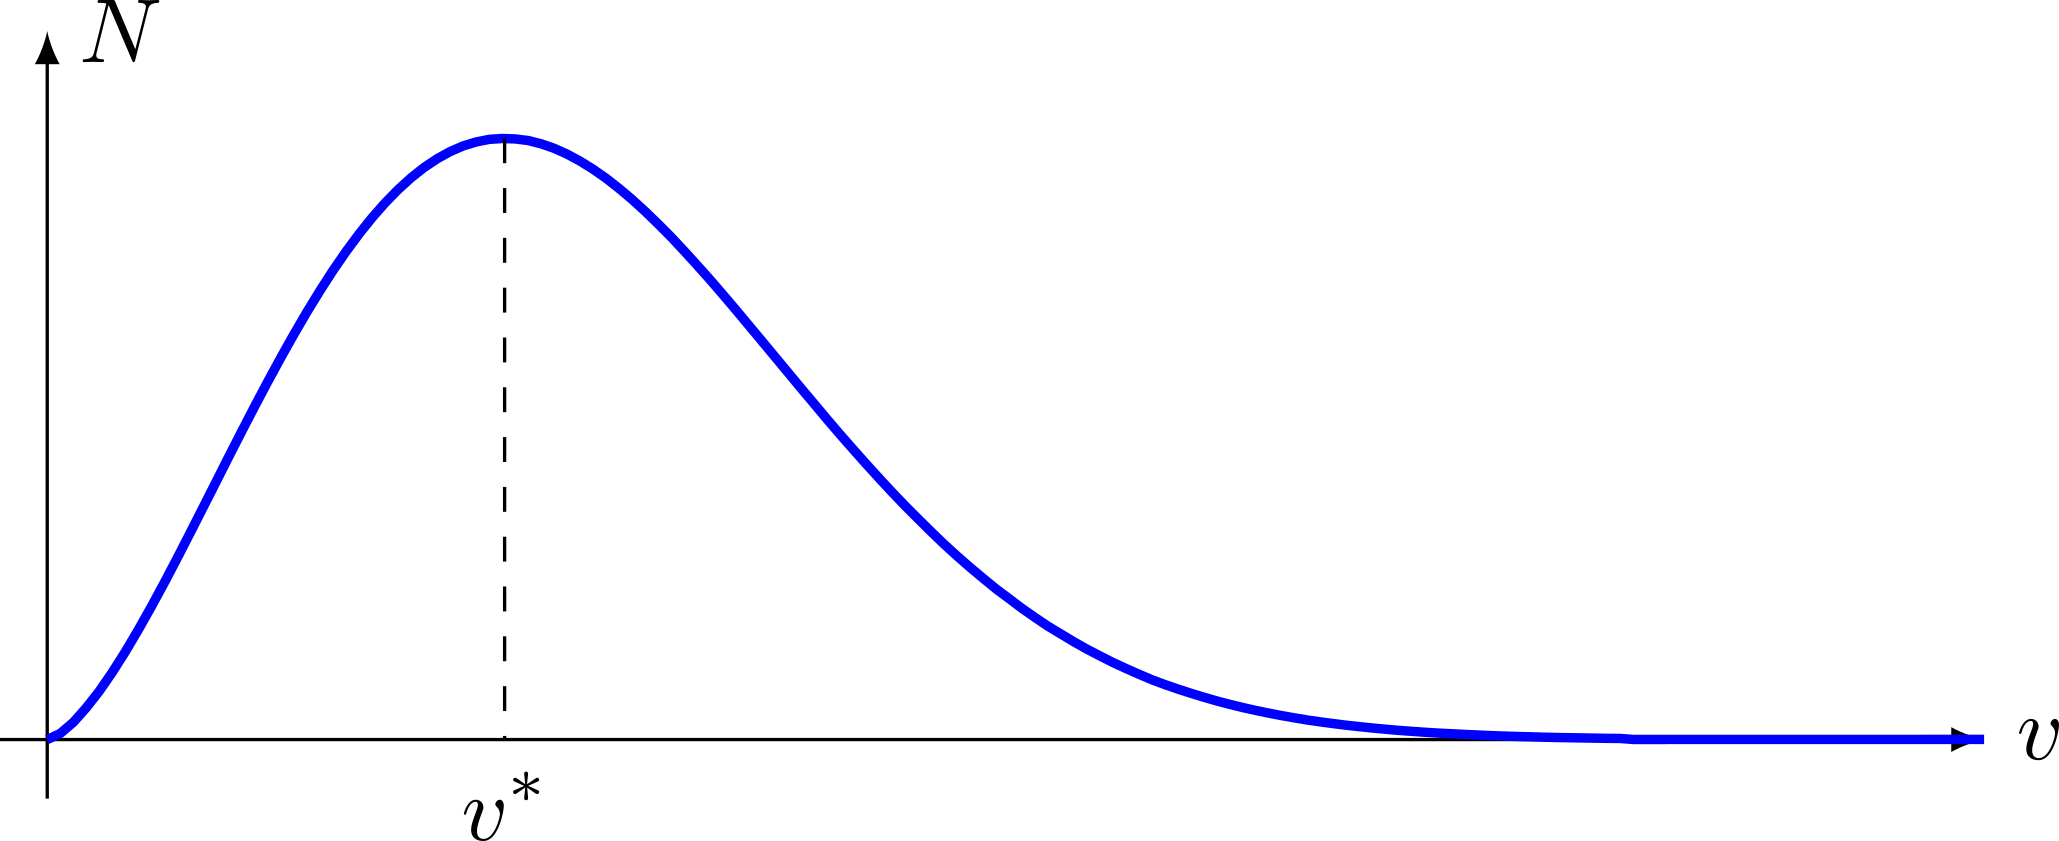
\includegraphics[height=3.5cm, draft=true]{arrh_vitesses}
	}{
		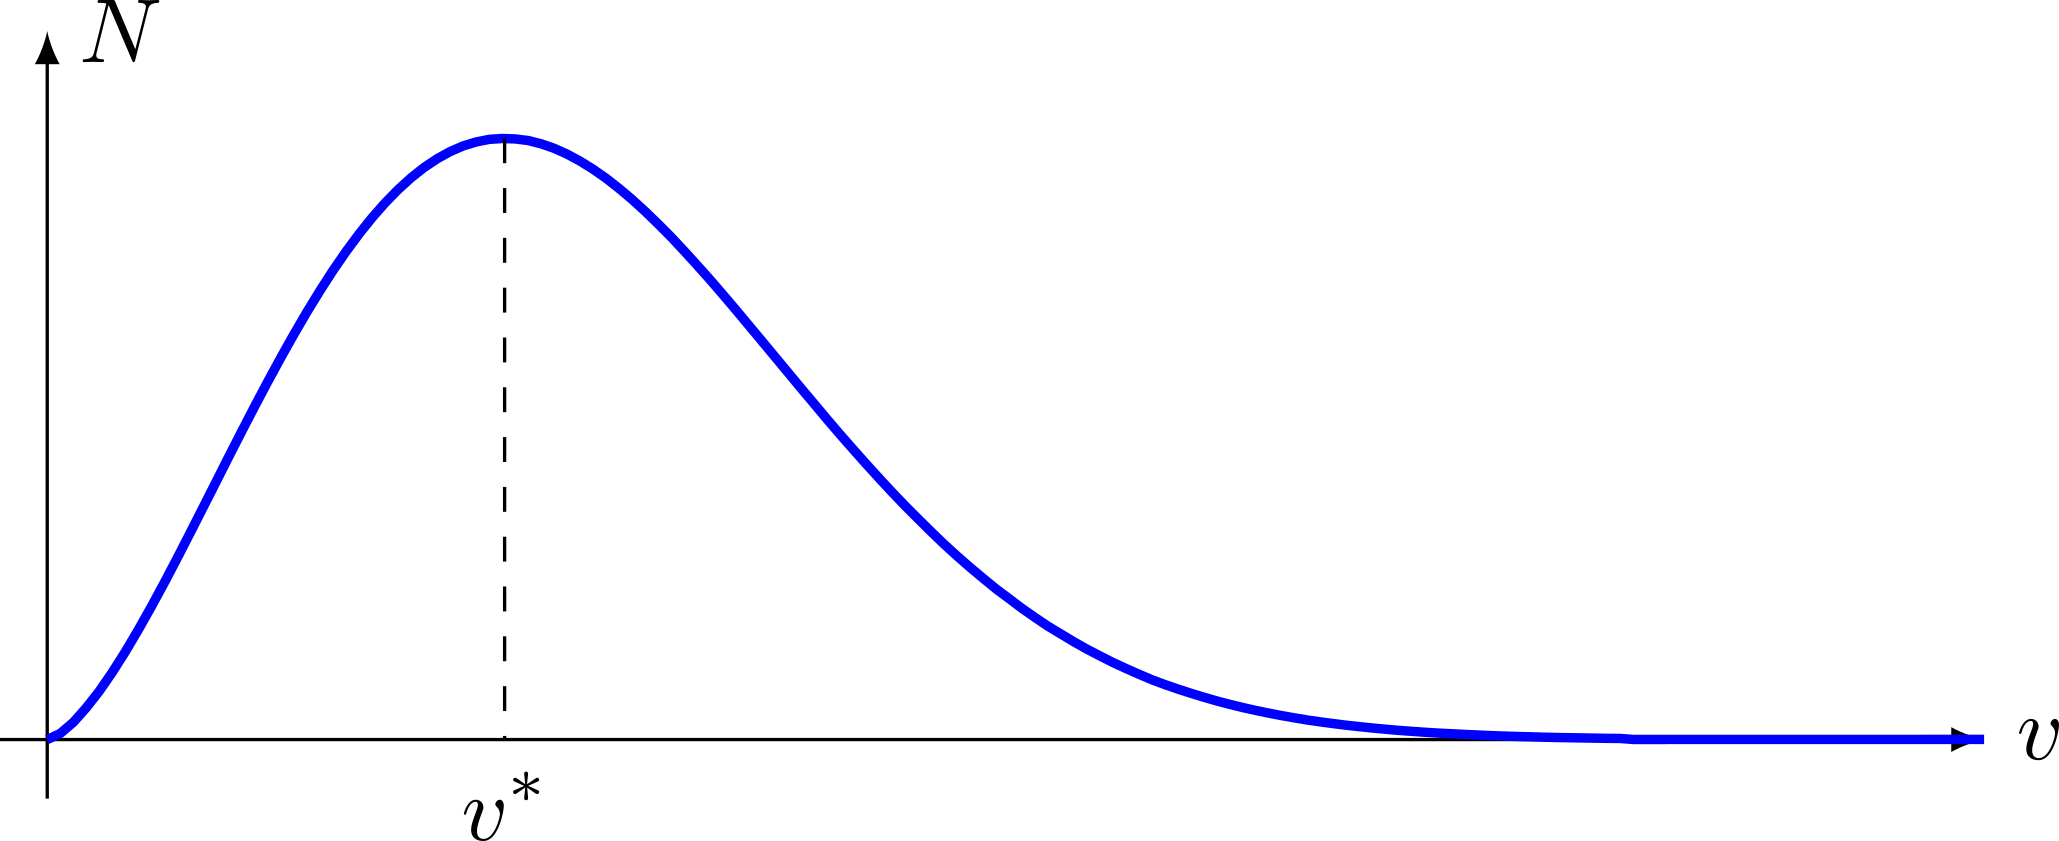
\includegraphics[height=3.5cm]{arrh_vitesses}
	}
	\captionof{figure}{Distribution des vitesses de molécules.}
\end{minipage}
\hfill
\begin{minipage}{0.49\linewidth}
	\sswitch{
		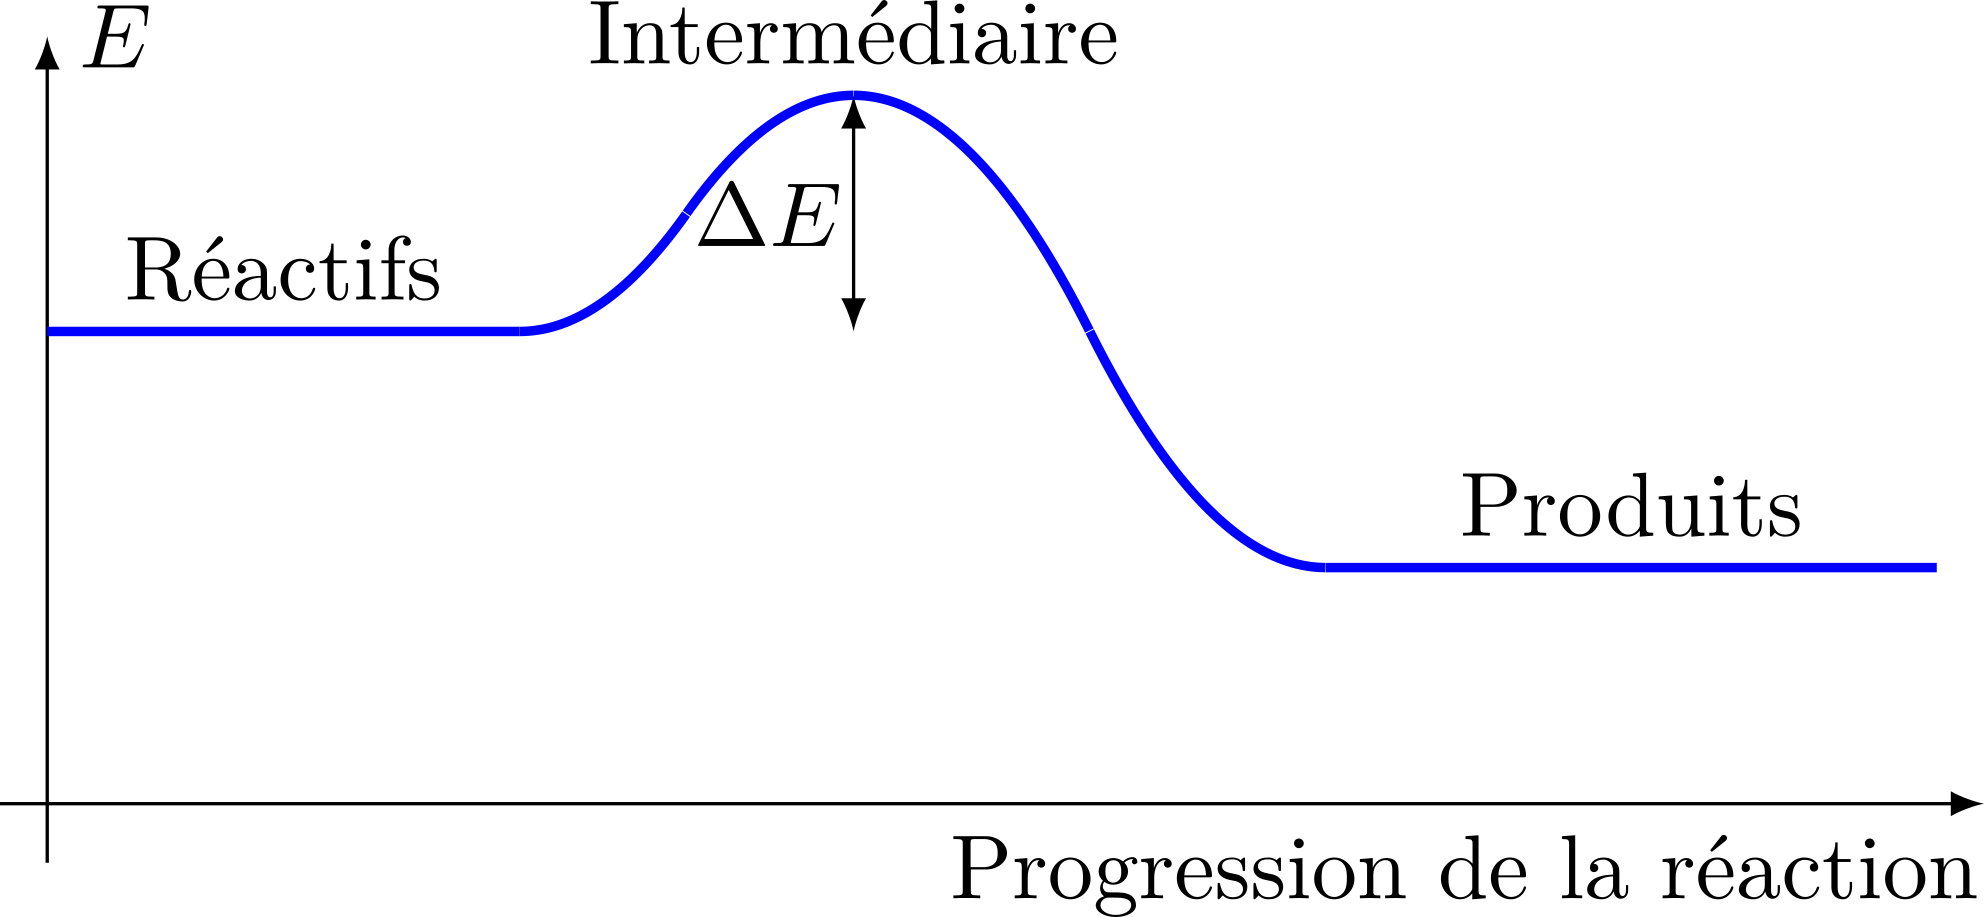
\includegraphics[height=3.5cm, draft=true]{arrh_ea}
	}{
		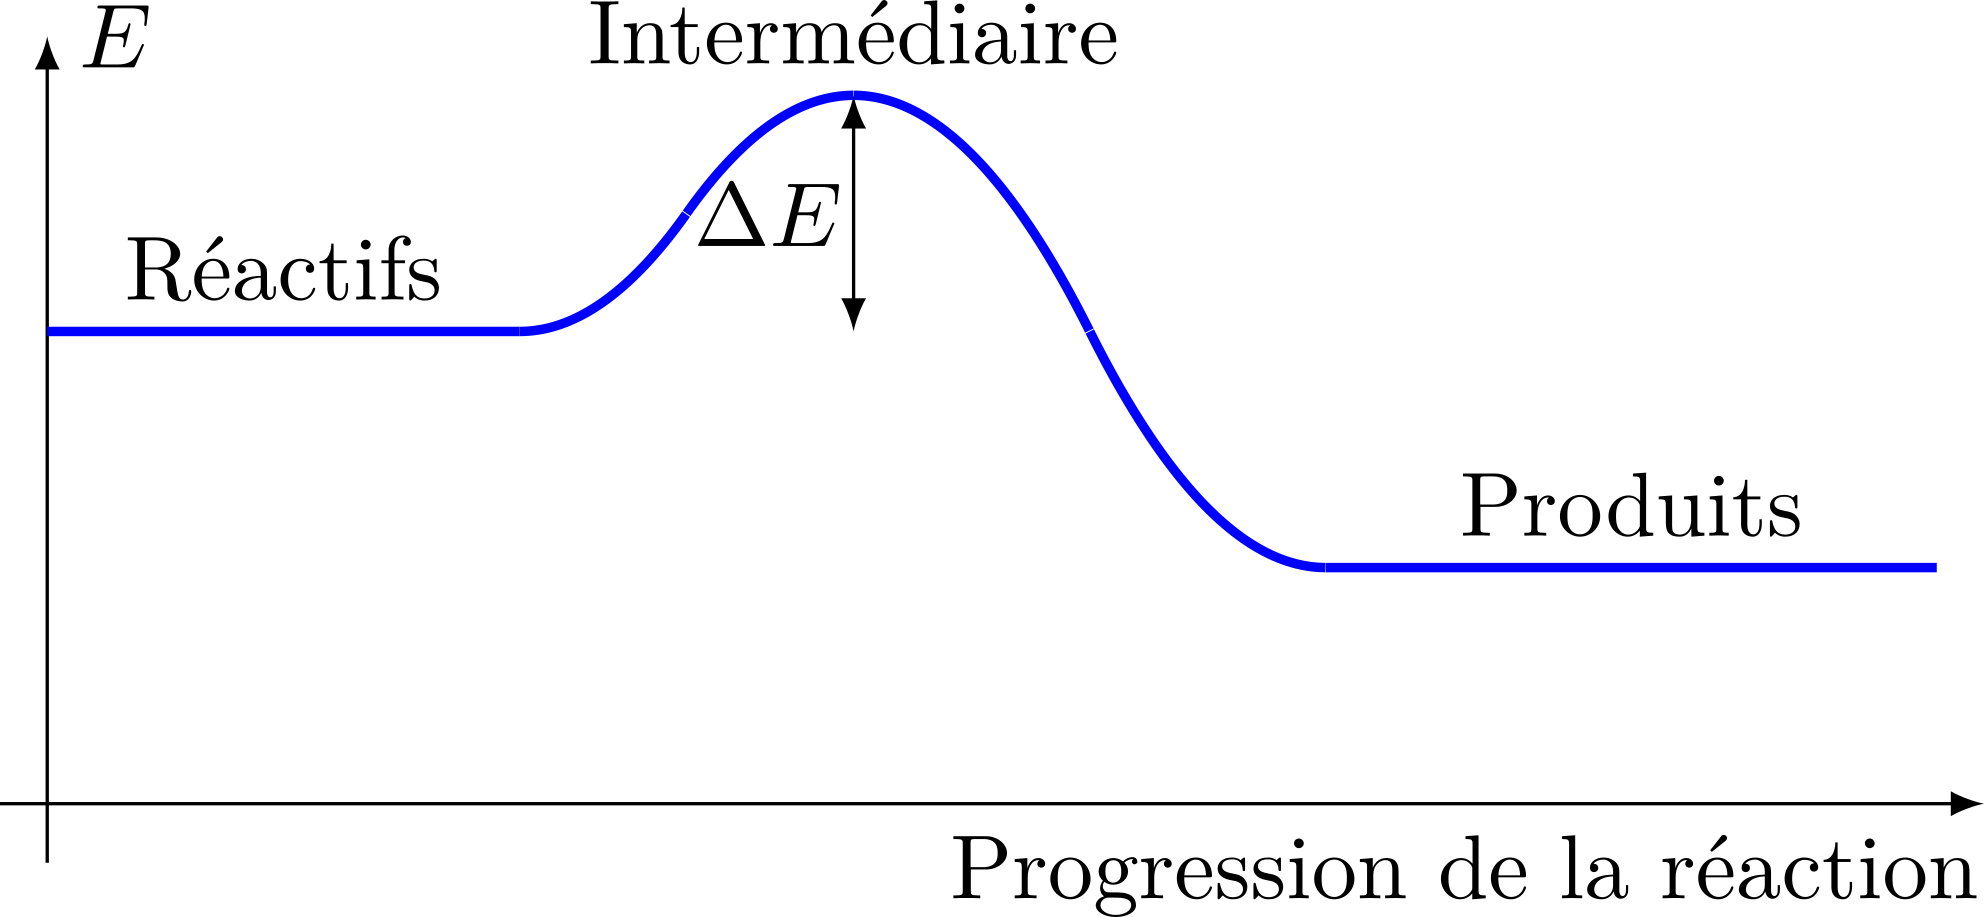
\includegraphics[height=3.5cm]{arrh_ea}
	}
	\captionof{figure}{Barrière d'activation chimique}
\end{minipage}

Plus la température est élevée, plus la proportion de molécules pouvant passer
cette barrière est élevée.

\subsection{Loi et utilisations}

L'évolution de la constante de vitesse suit une loi analytique en fonction de la
température, appelée \textbf{loi d'Arrhénius}~:
\begin{tcb}[label=loi:arrhenius, breakable](loi){Loi d'\textsc{Arrhénius}}
	La constante de vitesse d'une réaction chimique vérifie la loi empirique
	d'\textsc{Arrhénius}~:
	\psw{
		\[\boxed{k(T) = A\exp \left( - \frac{E_a}{RT} \right)}\]
	}
	\begin{itemize}
		\item \psw{
			      $A$ est le facteur pré-exponentiel, de même unité que $k$~;
		      }
		\item \psw{
			      $E_a$ est une grandeur positive appelée \textbf{énergie d'activation},
			      en $\si{J.mol^{-1}}$~;
		      }
		\item \psw{
			      $R$ est la constante des gaz parfaits, et $T$ la température en Kelvins.
		      }
	\end{itemize}
\end{tcb}

\subsubsection{Deux températures}

On peut utiliser cette loi pour trouver l'énergie d'activation d'une réaction,
ou à l'inverse déterminer la constante de vitesse d'une réaction. Dans le
premier cas par exemple, supposons qu'on a effectué le suivi cinétique d'une
même réaction à deux températures, $T_1$ et $T_2$, et déterminé $k(T_1)$ et
$k(T_2)$. D'après la loi d'\textsc{Arrhénius}, on a donc
\psw{
	\begin{gather*}
		\frac{k(T_1)}{k(T_2)}
		= \frac{A \exp \left( - \dfrac{E_a}{RT_1} \right)}{A
			\exp \left( - \dfrac{E_a}{RT_2} \right)}
		= \exp \left( \frac{E_a}{R} \left(
			\frac{1}{T_2} - \frac{1}{T_1} \right) \right)
		\\\Lra
		\boxed{E_a = R \frac{T_1T_2}{T_1-T_2}\ln \left( \frac{k(T_1)}{k(T_2)} \right)}
	\end{gather*}
}

\subsubsection{Succession de températures}
Avec une succession de températures, on peut tracer la régression linéaire~:
\psw{
	\[
		y\tikzmark{yn} = a\tikzmark{an}x\tikzmark{xn} + b\tikzmark{bn}
	\]
	\tikz[remember picture, overlay]
	\draw[-stealth, transform canvas={xshift=-6pt, yshift=-6pt}]
	(pic cs:yn) --++ (-10pt,-10pt)
	node[anchor=north east] {$\ln (k(T))$}
	;
	\tikz[remember picture, overlay]
	\draw[-stealth, transform canvas={xshift=-5pt, yshift=-6pt}]
	(pic cs:an) --++(-5pt,-10pt)
	node[anchor=north] {$-\frac{E_a}{R}$}
	;
	\tikz[remember picture, overlay]
	\draw[-stealth, transform canvas={xshift=0pt, yshift=-6pt}]
	(pic cs:xn) --++(5pt,-10pt)
	node[anchor=north] {$\frac{1}{T}$}
	;
	\tikz[remember picture, overlay]
	\draw[-stealth, transform canvas={xshift=3pt, yshift=-6pt}]
	(pic cs:bn) --++(10pt,-10pt)
	node[anchor=north west] {$\ln (A)$}
	;
}

\begin{tcb}*(expe)<itc>"trans"{Transition}
	Comment faisons nous en pratique un suivi expérimental, et notamment quelles
	sont les lois mathématiques derrière les suivis par grandeurs physiques~?
\end{tcb}

\section{Méthodes de suivi cinétique expérimental}
\subsection{Dosage par titrage}
\subsubsection{Définition}
\begin{tcb}[label=def:titrage](defi){Suivi cinétique par titrage}
	La méthode chimique consiste à prélever un faible volume d'essai du système
	étudié à intervalles de temps régulier~; la concentration des espèces
	chimiques d'intérêt est alors \textbf{titrée} sur ce volume d'essai.
\end{tcb}
Les méthodes de titrage seront détailles avec plus de précision plus tard dans
l'année, à la fois en cours et en TP. Ce qu'il faut en retenir pour le moment,
c'est qu'elle permet une détermination \textbf{absolue} de la concentration,
mais qu'elle présente certains forts désavantages~: c'est une méthode
\begin{bolditemize}
	\item[destructive]~: chaque prélèvement diminue le volume du système
	initial et la quantité de matière de produit ou réactif selon la
	méthode~;
	\item[laborieuse]~: il faut faire autant de dosages que de points de
	mesures~;
	\item[non continue]~: on n'a accès qu'à un nombre limité de points de
	mesure~;
	\item[lente]~: un dosage prend, au mieux et environ \SI{5}{min}.
\end{bolditemize}
Il faut donc notamment \textbf{arrêter la réaction} dans le volume d'essai, pour
que le prélèvement à un instant $t$ dosé environ \SI{5}{min} plus tard
corresponde quand même à un point de mesure à l'instant $t$. Pour ce faire, il
faut avoir recours à une \textbf{trempe chimique}.

\subsubsection{La trempe chimique}
La trempe chimique est le nom d'un processus destiné à figer l'état d'un
systèmes physico-chimiques. On recense trois méthodes de trempe~:
\begin{enumerate}
	\item \textbf{La dilution}~: la vitesse de réaction étant une fonction
	      croissante de la concentration en réactif, \textbf{diluer le volume
		      d'essai} d'un facteur 10 à 100 permet de ralentir fortement la cinétique
	      de la réaction.
	\item \textbf{Le refroidissement}~: la constante de vitesse croît avec la
	      température, et par conséquent abaisser la température du volume d'essai
	      permet de ralentir la cinétique de la réaction qui s'y passe. C'est une
	      méthode particulièrement intéressante quand on part de réactions
	      initialement hautes en températures, pour abaisser par exemple de
	      \SI{100}{\degreeCelsius} à \SI{0}{\degreeCelsius} la solution.
	\item \textbf{La disparition d'un réactif}~: il est également possible de
	      faire disparaître l'un des réactifs (celui qui ne sera pas dosé) en
	      réalisant une réaction rapide et totale avant d'effectuer le dosage. Par
	      exemple, une réaction ayant pour réactif un acide peut être interrompue
	      en modifiant le pH du volume par ajout d'une base forte, comme
	      $\ce{HO-}$.
\end{enumerate}

\subsection{Dosage par étalonnage}
Comme introduit dans la première section, il est possible de sonder
indirectement la concentration en une espèce \textit{via} l'évolution d'une
grandeur physique. Pour que le suivi soit quantitatif, il faut que la valeur de
la grandeur mesurée soit comparée à une valeur de référence, un étalon. Pour
qu'un dosage par étalonnage soit efficace, il faut~:
\begin{itemize}
	\item que la grandeur évolue de manière sensible lorsque l'on passe du
	      réactif au produit. Si le réactif a la même conductivité que le produit
	      formé, on comprend aisément qu'un suivi conductimétrique ne nous sera
	      d'aucune aide…
	\item que la grandeur varie de manière simple et prédictible avec la
	      concentration (si possible de manière linéaire).
\end{itemize}

\subsubsection{Spectrophotométrie}
\begin{tcb}[label=loi:berrlambert](loi){Loi de \textsc{Beer-Lambert}}
	On relie l'intensité lumineuse transmise par une espèce à une longueur
	d'onde donnée avec la concentration de l'espèce colorée en solution grâce à
	la loi de \textbf{Beer-Lambert}~:
	\[
		\boxed{
			A = \log \left( \frac{I_0}{I} \right) = \sum_{i=1}^{N}\epsilon_i
			\ell c_i
		}
	\]
	\begin{itemize}
		\item $A$ est l'\textbf{absorbance}, sans dimension~;
		\item $I_0$ l'intensité lumineuse \textbf{incidente}, en $\si{W.m^{-2}}$~;
		\item $I$ l'intensité lumineuse \textbf{en sortie}, aussi en
		      $\si{W.m^{-2}}$~;
		\item $\epsilon_i$ le coefficient d'extinction molaire de l'espèce X$_i$
		      à la longueur d'onde $\lambda$ (dépend de l'espèce et un peu du
		      solvant et de $T$)~;
		\item $\ell$ la distance traversée par le faisceau, en \si{m} (souvent
		      \si{cm})~;
		\item $c$ la concentration de l'espèce absorbante X$_i$, en
		      $\si{mol.L^{-1}}$.
	\end{itemize}
	\begin{center}
		C'est une loi \textbf{additive} et \textbf{linéaire}.
	\end{center}
\end{tcb}

\subsubsection{Conductimétrie}
\begin{tcb}[label=loi:kohlrausch](loi){Loi de \textsc{Kohlrausch}}
	Les ions conduisant le courant, il est possible dans certains cas de suivre
	l'avancement de la réaction en mesurant l'évolution de la conductivité de la
	solution associée à la concentration des ions grâce à la \textbf{loi de
		Kohlrausch}~:
	\[\boxed{\sigma = \sum_{i=1}^{N}\lambda_ic_i}\]
	\begin{itemize}
		\item $\sigma$ est la conductivité de la solution, en
		      $\si{\Omega^{-1}.m^{-1}}$~;
		\item $\lambda_i$ est la conductivité molaire ionique de l'espèce X$_i$,
		      dépendante de l'espèce et de la température, en
		      $\si{\Omega^{-1}.m^{-1}.mol^{-1}.L}$~;
		\item $c_i$ est la concentration molaire en l'espèce X$_i$, en
		      $\si{mol.L^{-1}}$.
	\end{itemize}
	\begin{center}
		C'est une loi \textbf{additive} et \textbf{linéaire}.
	\end{center}
\end{tcb}

\end{document}
